%-------------------------------------------------------------------
\chapter{Implementation}
\label{c:implementation}
%-------------------------------------------------------------------

\epigraph{\enquote{Sometimes, the elegant implementation is just a function. Not a method. Not a class. Not a framework. Just a function.}}{\emph{John Carmack}}

This chapter shows the details of the implementation of the work.

%----------------------------------------------------------
\section{How experiments are structured}
%----------------------------------------------------------

The experimental work in this thesis is organized as a sequence of increasingly controlled studies.
The main research question is whether increasing the \emph{spatial neighborhood size} (\(NB\)) in Mixture Neural Cellular Automata improves long-horizon behavior in a tissue-growth setting.
In practice, the experiments are implemented as training/evaluation pipelines that can be repeated across multiple neighborhood sizes, while keeping all other hyperparameters fixed whenever possible.

At a high level, each experiment follows the same steps:
\begin{itemize}
\item generate or load a dataset of tissue-growth trajectories (``histories'');
\item train one or more NCA variants on short temporal windows extracted from these histories;
\item evaluate the trained models by running free rollouts (no teacher forcing) for different horizons;
\item compute quantitative metrics and inspect qualitative rollouts.
\end{itemize}

%----------------------------------------------------------
\section{Data generation and biological toy model}
%----------------------------------------------------------

Before training NCAs, we need supervised trajectories representing plausible tissue dynamics.
In this thesis, these trajectories are generated by a simple stochastic, biologically-inspired simulator and collected through a small data-generation pipeline.

\paragraph{State representation (cell types).}
Each simulation state is a 2D grid of discrete cell types.
In the ``complex'' configuration used for most experiments, the simulator includes a small differentiation hierarchy (e.g., \texttt{STEM}, \texttt{INTERMEDIATE}, and \texttt{DIFFERENTIATED} types), plus an \texttt{EMPTY} background.

\paragraph{Local update rules (biological intuition).}
At each simulation step, each occupied cell can:
(i) die, (ii) survive, or (iii) divide into a nearby empty site.
When a division happens, the newly created cell may \emph{differentiate} according to a probability table that depends on the parent cell type and (optionally) on neighbor context.
This yields trajectories that show growth, spatial organization, and gradual maturation into differentiated compartments.

\paragraph{Histories.}
For a single simulation we record the entire time series of grids \(x_0, x_1, \dots, x_T\).
We refer to this time series as a \emph{history}.
In the thesis we may visualize a history either as a sequence of snapshots (selected time points) or as a small montage, because it helps identify qualitative behaviors (stable growth, collapse, frozen patterns, etc.).

\paragraph{Dataset definition.}
Formally, the dataset is a collection of histories:
\[
\mathcal{D}=\{x^{(i)}_{0:T}\}_{i=1}^{N},
\]
where each \(x^{(i)}_t\) is a discrete 2D grid state at time \(t\).
In this work we use multiple datasets with different \(N\) and \(T\) depending on the experiment.

\paragraph{How a single history is generated (example).}
To generate one history, we start from an initial condition where a small cluster of stem-like cells is placed near the center of the grid (with small randomness), while all other sites are empty.
Then, for each time step, cells update locally:
each occupied site may die, survive, or divide into a nearby empty site; if a division occurs, the newly created cell may differentiate according to a type-dependent probability table that can also be influenced by the local neighborhood composition.

The goal is not to perfectly match biology, but to produce trajectories with growth and spatial organization that can serve as supervised targets for learning a local update rule.

\begin{figure}[t]
  \centering
  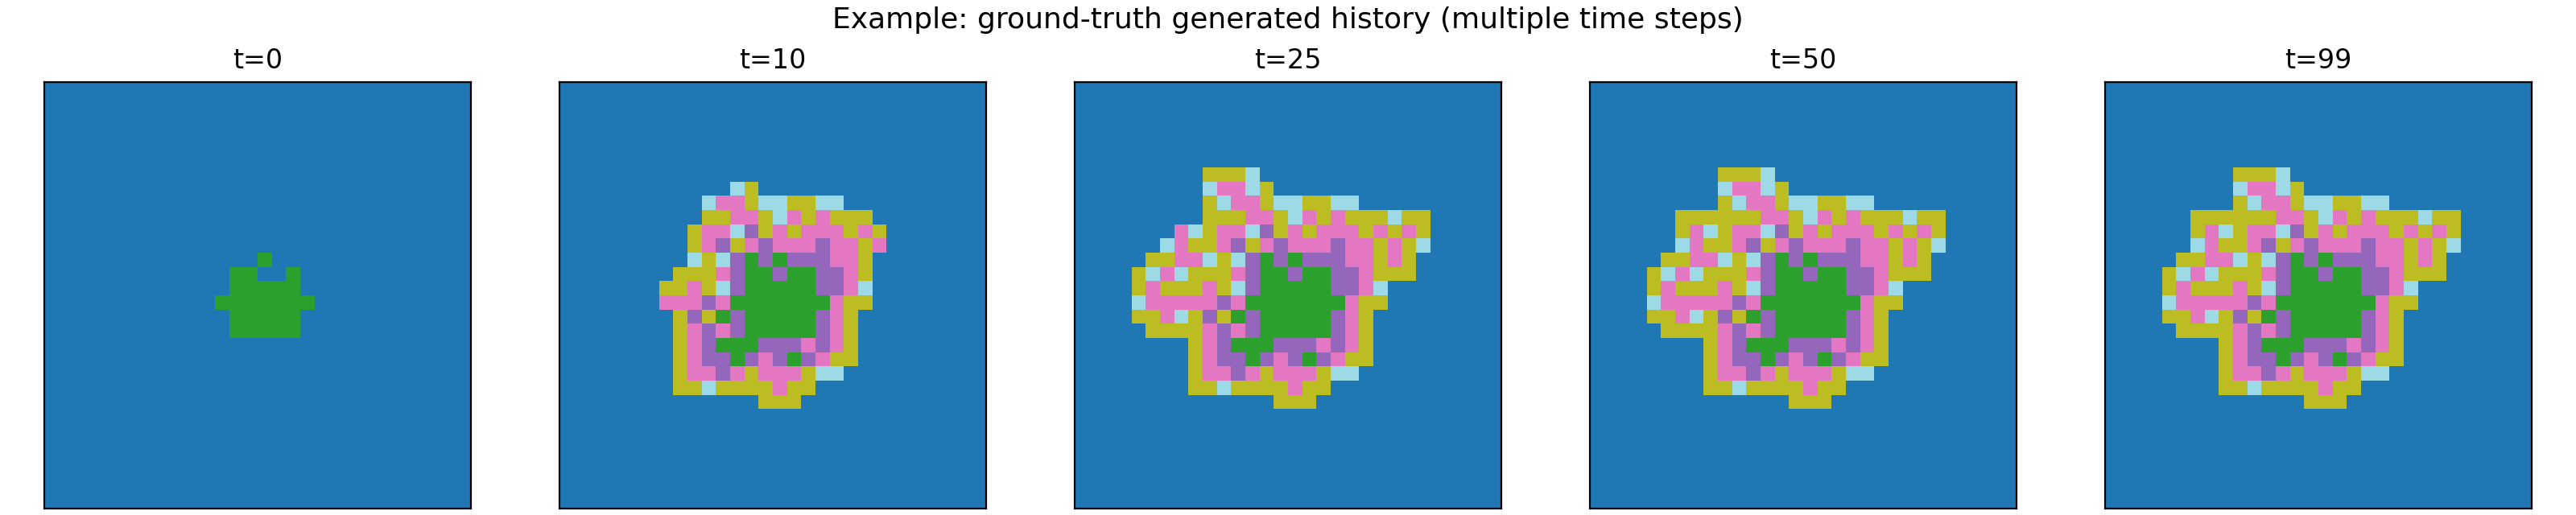
\includegraphics[width=\textwidth]{figs/tissue_examples/history_generation_example.png}
  \caption{Example of a generated history (ground truth) shown at multiple time steps. Each panel is a snapshot of the same simulation at a different time point.}
  \label{fig:impl:data:history_example}
\end{figure}

\paragraph{Datasets used in this thesis.}
Different experiments used different history datasets.
For instance, the final neighborhood sweep uses a dataset of 300 simulated trajectories with a horizon of 100 time steps (stored as a serialized array for reproducibility).

%----------------------------------------------------------
\section{Model training: from trajectories to learned update rules}
%----------------------------------------------------------

All NCA-style models in this thesis learn a \emph{local} update rule that is applied repeatedly over time.
Conceptually, a standard formulation is:
\begin{equation}
x_{t+1} = x_t + f_{\theta}\!\left(\mathcal{P}(x_t)\right),
\end{equation}
where \(x_t\) is the grid state at time \(t\), \(\mathcal{P}(\cdot)\) is a local perception operator (it extracts neighborhood information), and \(f_{\theta}\) is a neural network that predicts an update.
Mixture models extend this idea by having multiple candidate update rules and a learned mechanism to select (or mix) them over space and time \cite{mnca_milite2025}.

In training, the models are usually optimized on short temporal windows extracted from longer histories (teacher-forced supervision), while evaluation is performed as free-running rollouts.
This gap is important when we compare neighborhood sizes, because a low short-horizon loss does not automatically imply stable long-horizon behavior.

\paragraph{Example of generation by the learned model (multi-step rollout).}
After training, we can use a model to generate a trajectory by starting from an initial grid \(x_0\) and iterating the learned update rule for multiple steps, producing \(\hat{x}_1, \hat{x}_2, \dots, \hat{x}_T\).
Figure~\ref{fig:impl:model:rollout_example} shows an example rollout over multiple steps (same initial condition as \cref{fig:impl:data:history_example}), illustrating what it means for the model to ``free-run''.

\begin{figure}[t]
  \centering
  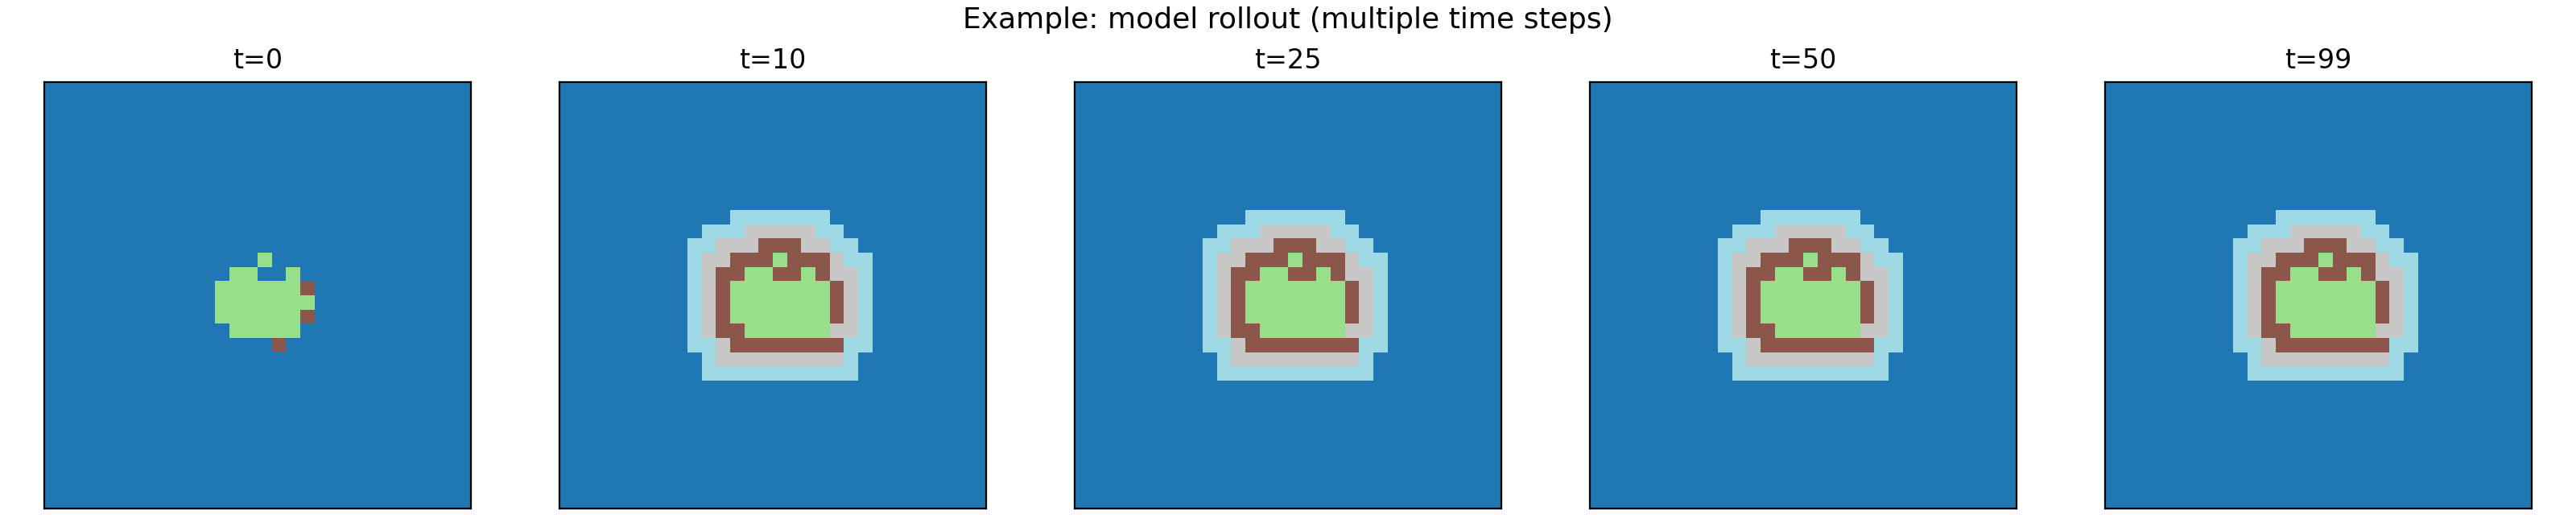
\includegraphics[width=\textwidth]{figs/tissue_examples/model_rollout_example.png}
  \caption{Example of a model-generated rollout over multiple steps, starting from the same initial condition used for the ground-truth history. This visualization helps qualitatively assess whether the learned dynamics remain stable when the model is run freely.}
  \label{fig:impl:model:rollout_example}
\end{figure}

\begin{figure}[t]
  \centering
  \begin{minipage}[t]{0.49\textwidth}
    \centering
    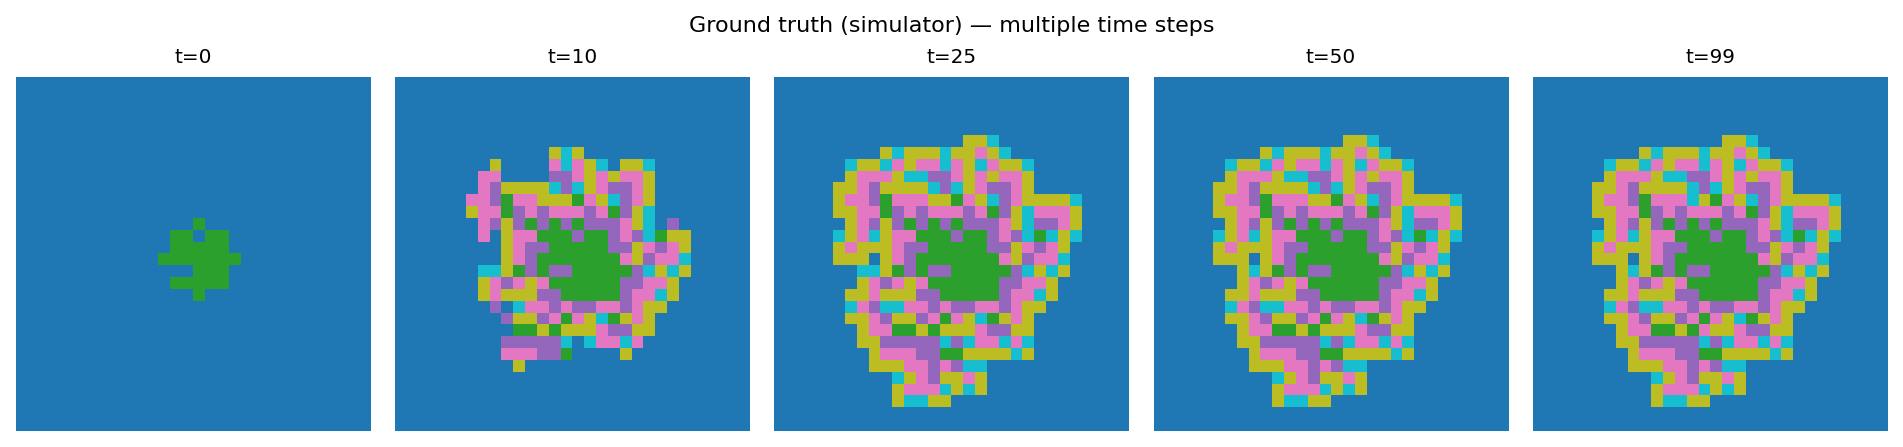
\includegraphics[width=\textwidth]{../presentation/assets/same_init/sample_149/ground_truth.png}
    
    {\small \textbf{Ground truth (simulator)}}
  \end{minipage}\hfill
  \begin{minipage}[t]{0.49\textwidth}
    \centering
    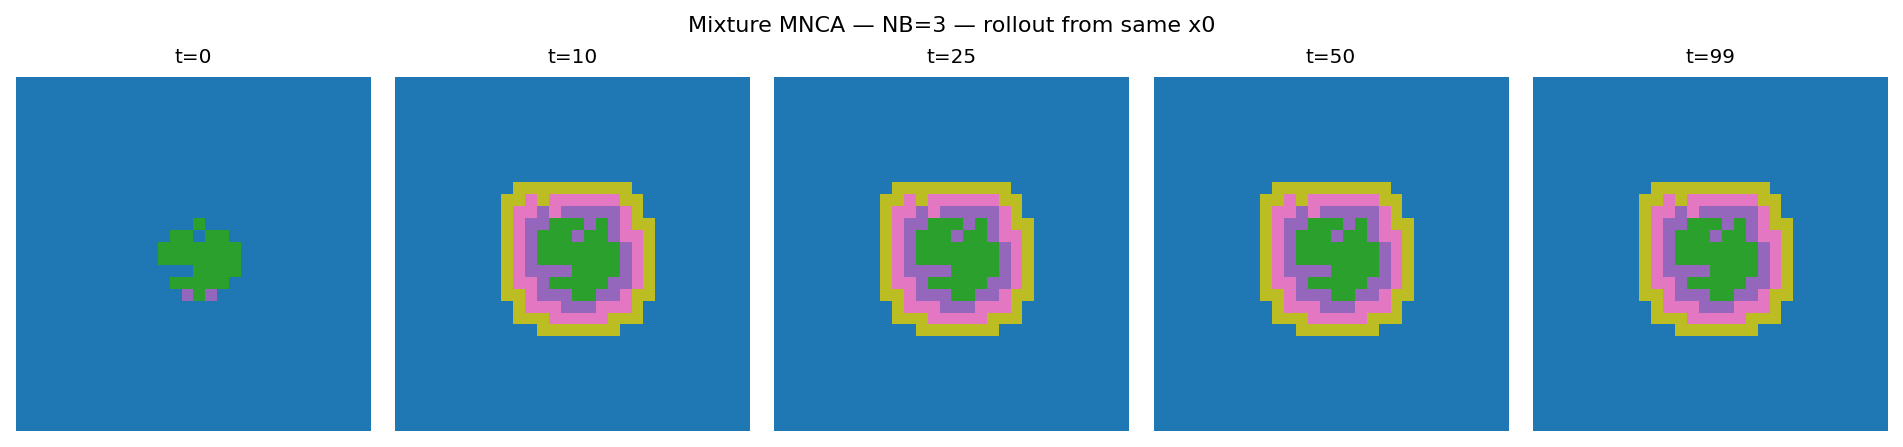
\includegraphics[width=\textwidth]{../presentation/assets/same_init/sample_149/mixture_nb_3.png}
    
    {\small \textbf{Model rollout (Mixture MNCA, NB=3)}}
  \end{minipage}
  \caption{Qualitative comparison on the same initial condition (sample 149): ground truth simulator history vs model-generated rollout. Both start from the exact same $t=0$ state.}
  \label{fig:impl:gt_vs_model_side_by_side}
\end{figure}

%----------------------------------------------------------
\section{Reference experimental setting from the original MNCA paper}
%----------------------------------------------------------

The starting point for our experiments is the training protocol used in the reference MNCA paper \cite{mnca_milite2025}.
In its ``paper-like'' regime, training uses a relatively small dataset and a short temporal horizon, with a long optimization schedule.
We replicate this setting as closely as possible and then change only the neighborhood size \(NB\), to isolate its effect.

%----------------------------------------------------------
\section{Experiment: does it make sense to extend the neighborhood?}
%----------------------------------------------------------

Our first experiment had a simple goal: understand whether extending the spatial neighborhood in MNCA is a meaningful direction.
We initially followed the paper-like regime, and then progressively changed the data and training schedule to strengthen supervision and make long-horizon training feasible.
Overall, the experiment was carried out in three steps (three configurations).

\subsection{Summary of steps 1 and 2}

We started from the training setup used in the reference paper: a relatively small dataset (\textbf{200 simulated trajectories}) with a short temporal horizon (\textbf{35 time steps}) trained for \textbf{800 epochs}.
Our first goal was not to change the learning procedure itself, but to isolate the effect of the \emph{spatial neighborhood size} (NB) by repeating the same training protocol across multiple neighborhoods.
In principle, increasing NB should allow the update rule to condition on a broader spatial context, which could improve regeneration and pattern stability.

In practice, this ``paper-like'' regime did not produce a clean answer to the neighborhood question.
Across several NB values, the qualitative rollouts remained inconsistent and the quantitative differences were small, making it hard to tell whether (i) NB genuinely had little impact, or (ii) the training signal was simply too weak/noisy in this low-data, short-horizon setting.
At that point, we were not confident that a negative result would be meaningful.

Following this, we attempted to strengthen the supervision by increasing both dataset size and sequence length, moving to \textbf{1000 trajectories of 500 time steps} each.
The motivation was twofold: (1) more trajectories reduce variance and improve coverage of initial conditions, and (2) longer sequences better represent the long-horizon behavior we ultimately care about when judging whether a model ``regenerates'' rather than just matching short-term transitions.
However, training directly on long sequences at this scale was computationally heavy and slowed iteration substantially.

To make long-horizon training feasible, we introduced \textbf{curriculum learning}, training on progressively longer temporal windows (e.g., a first phase with a \textbf{35-step} window, then \textbf{100-step}, and finally \textbf{500-step}, with fewer epochs and smaller learning rates in later phases).
The intended effect of the curriculum was to let the models first learn stable short-term local dynamics and then refine them under longer-horizon constraints without paying the full cost of long unrolls from the beginning.

Despite the curriculum, the resulting rollouts were often poor (the tissue failed to regenerate convincingly), which again prevented a meaningful comparison across neighborhood sizes.
At this stage we revisited the experimental pipeline and concluded that the main problem was not simply ``insufficient compute'', but \textbf{confounding factors that made the neighborhood sweep hard to interpret when the models were already failing}.
In particular, when training is dominated by short teacher-forced transitions while evaluation is performed as free-running rollouts, low training loss does not necessarily translate into good long-horizon behavior.
In addition, mixture models can behave very differently depending on whether rule selection is evaluated with soft (differentiable) assignments or hard sampling; if this is not kept consistent, the observed differences can be dominated by sampling behavior rather than by NB.

\subsection{Step 3: controlled neighborhood sweep (final configuration)}

For these reasons, we temporarily stepped back from the long-horizon curriculum experiment and adopted a more controlled ablation aimed specifically at answering the neighborhood-size question.
We fixed the ``extra'' degrees of freedom that can dominate dynamics (most importantly, keeping the rule-selection temperature effectively constant during the sweep and using a consistent sampling mode at evaluation), and we generated an intermediate dataset that is large enough for stability while still tractable (\textbf{300 trajectories, 100 time steps}).

We then evaluated each trained model at multiple rollout horizons (e.g., \textbf{25, 50, 100 steps}) rather than relying on a single horizon.
This produces a clearer picture: even if different NB values look similar at very short horizons, improvements from larger neighborhoods are expected to show up as slower degradation and better stability as the rollout length increases.

In summary, curriculum learning was introduced as a pragmatic response to the computational cost of training on \textbf{1000$\times$500} simulations.
We then reverted to a simpler setting not because the curriculum is ``wrong'', but because we first needed an interpretable experimental protocol where the neighborhood-size effect is not masked by optimization and sampling confounds.
Once a robust NB trend is established under controlled conditions, curriculum learning can be reintroduced as a second-stage validation on selected neighborhoods to confirm that the effect persists in the full long-horizon regime.

\paragraph{Where the results are reported.}
Since this configuration is part of the experimental \emph{pipeline design} (and it directly motivates our final protocol), we report its detailed results in this Implementation chapter.
The \cref{c:results} chapter instead focuses on the overall thesis conclusions.

\paragraph{High-level outcome (brief).}
Under this controlled protocol, the neighborhood-size effect becomes observable.
In our sweep over \(NB \in \{1,\dots,7\}\), \(NB=1\) is consistently inadequate, while moving to \(NB\ge2\) yields a clear improvement.
Beyond this first jump, improvements are not strictly monotonic: different neighborhood sizes trade off distributional agreement and spatial fidelity, and differences become more evident as the rollout horizon increases (e.g., 25 vs 100 steps).

%----------------------------------------------------------
\subsubsection{Step 3 results: evaluation protocol and key trends}
\label{sec:impl:step3:results}
%----------------------------------------------------------

We evaluate models trained with neighborhood sizes \(NB \in \{1,\dots,7\}\) using both \emph{distributional} and \emph{spatial} metrics computed on the final state of each generated simulation.
The reference dataset consists of 300 ground-truth histories with a horizon of 100 steps (stored as a serialized array for reproducibility).
For each neighborhood size, models are evaluated at multiple generation horizons (Step Length \(=25,50,100\)).
For each configuration we report aggregated performance (mean and variability across repeated evaluations) and we additionally inspect \emph{per-simulation} distributions to assess robustness and failure modes (heavy tails and outliers).

Figure~\ref{fig:impl:step3:dashboard} summarizes the overall trends across neighborhood sizes for the key metrics.
The main qualitative pattern is consistent across metrics: \(NB=1\) is systematically inadequate, while moving to \(NB\ge2\) yields a sharp performance improvement.
Beyond this first jump, increasing \(NB\) produces a non-monotonic trade-off between matching global distributions (e.g., KL divergence) and matching spatial structure (e.g., tumor size and border properties).

\begin{figure}[t]
  \centering
  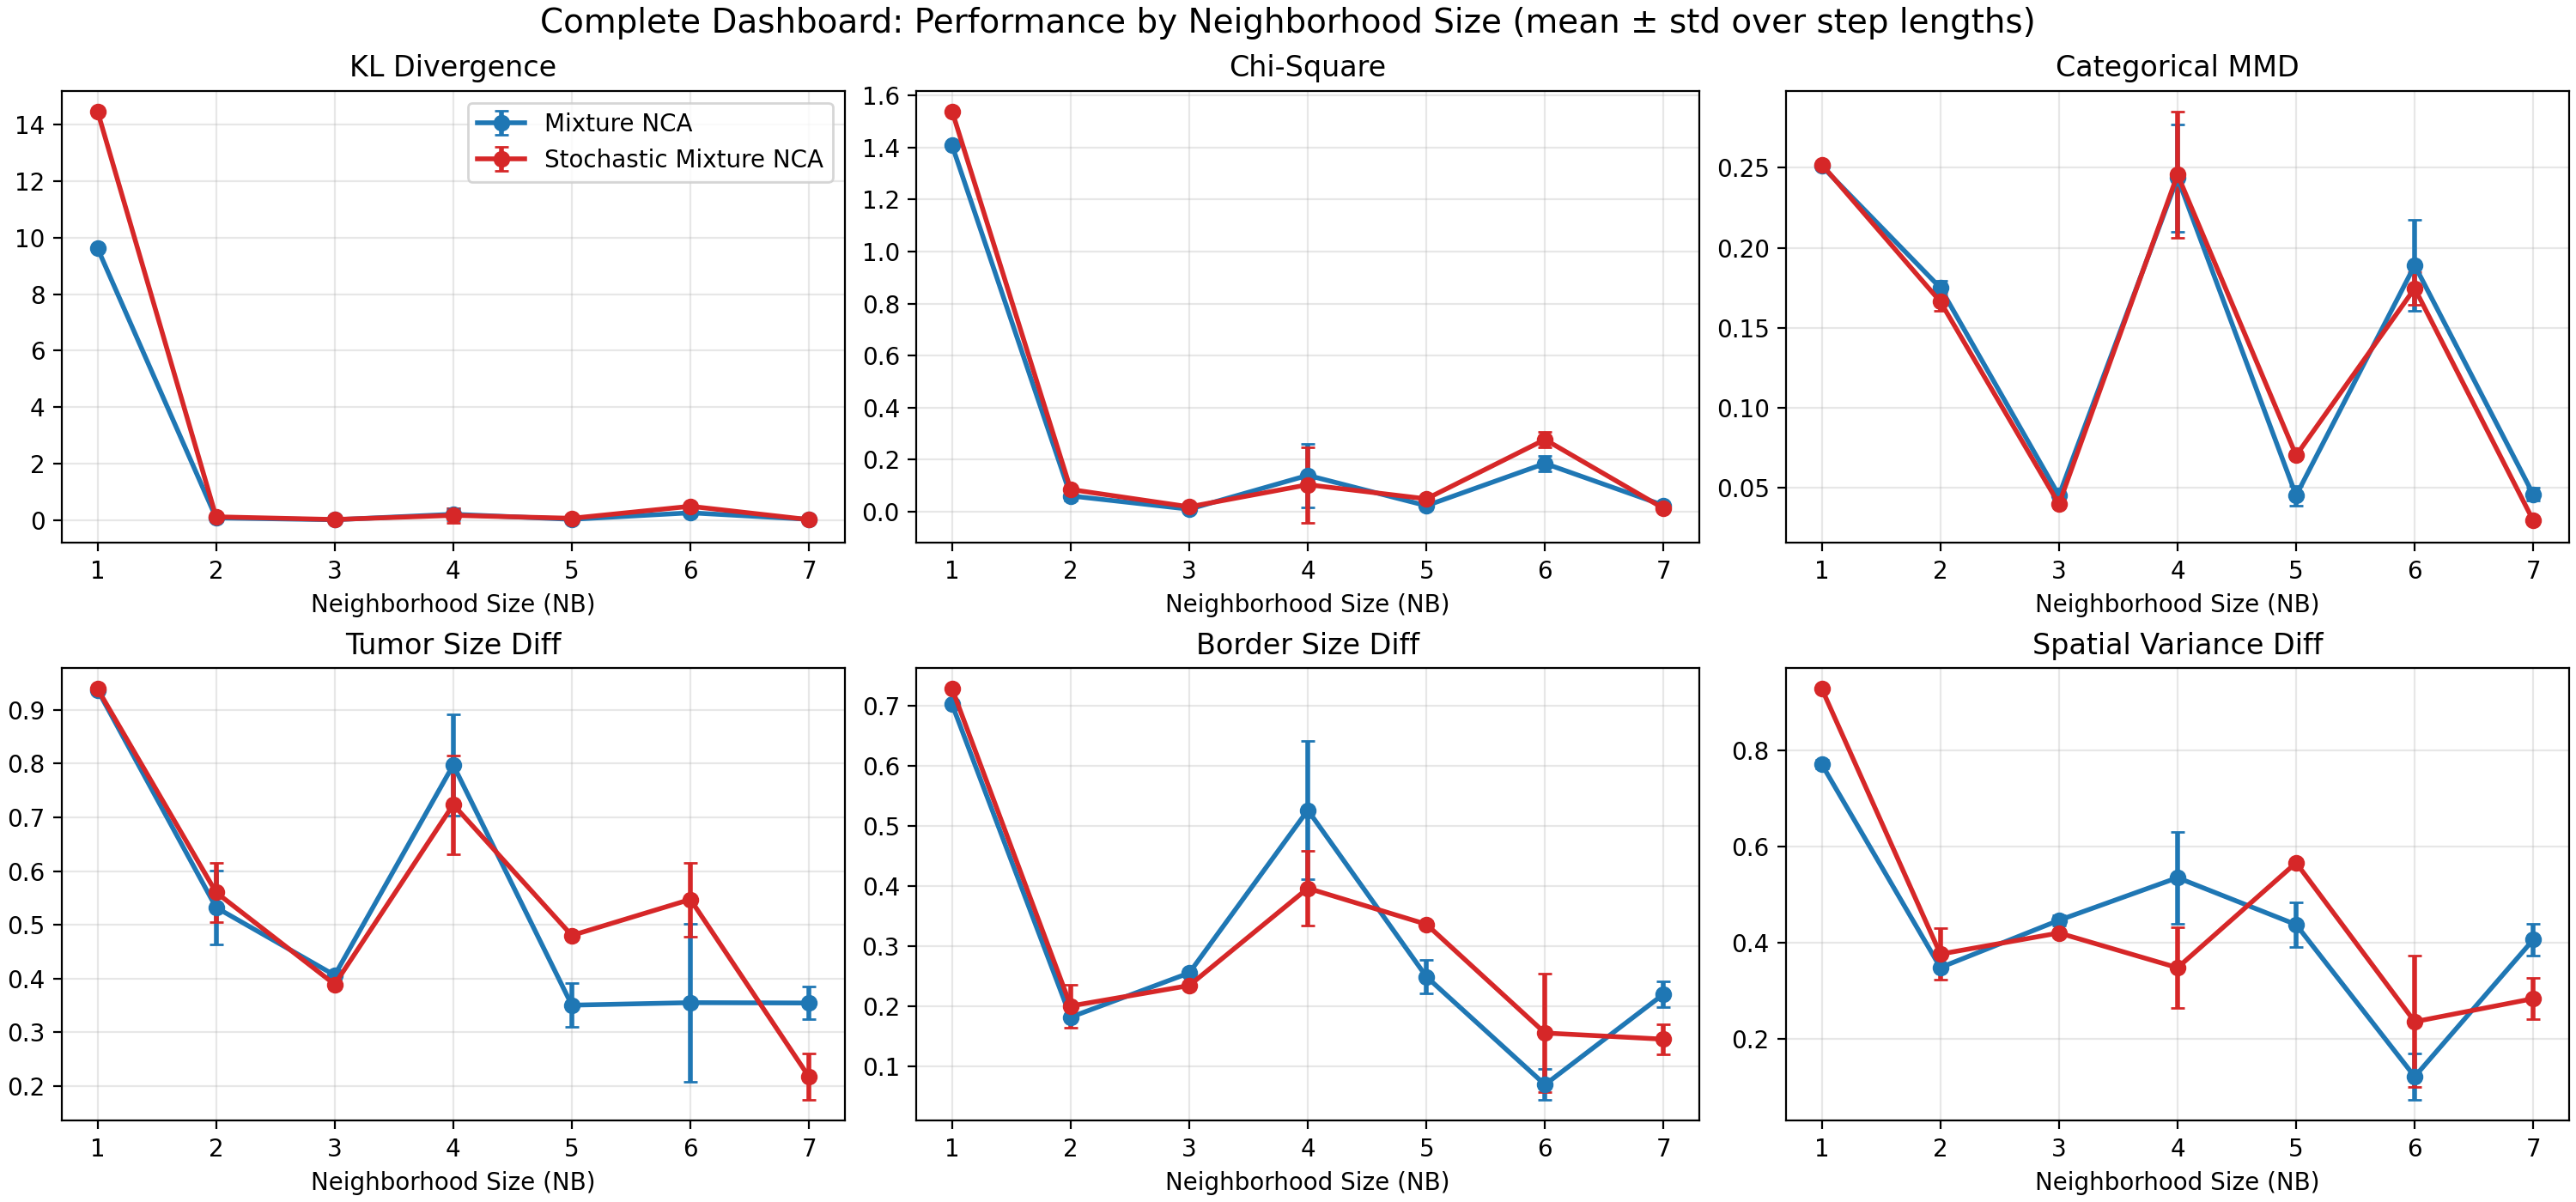
\includegraphics[width=\textwidth]{figs/neighborhood_analysis/nb_sweep_300x100/metrics_dashboard_full.png}
  \caption{Step 3: complete dashboard for the neighborhood sweep. We report mean and variability (standard deviation computed over the available step-length conditions) for the six metrics used in the analysis: KL divergence, Chi-square, categorical MMD, tumor size difference, border size difference, and spatial variance difference.}
  \label{fig:impl:step3:dashboard}
\end{figure}

%----------------------------------------------------------
\subsubsection{Distributional agreement and per-simulation variability}
\label{sec:impl:step3:kl}
%----------------------------------------------------------

KL divergence captures how well the global composition of cell types in the generated final state matches the empirical distribution from the dataset.
Across all step lengths, \(NB=1\) yields very large KL values, indicating a strong mismatch in global composition.
For \(NB\ge2\), both models reach low KL on average, but the best neighborhood can depend on the evaluation horizon and on whether rule selection is deterministic or stochastic.

To interpret robustness, we inspect \emph{per-simulation} distributions of the metrics using violin plots.
Compared to mean-only summaries, violins reveal heavy tails and outliers: these correspond to runs that converge to qualitatively wrong outcomes (failure modes), even when the median performance is competitive.

\begin{figure}[t]
  \centering
  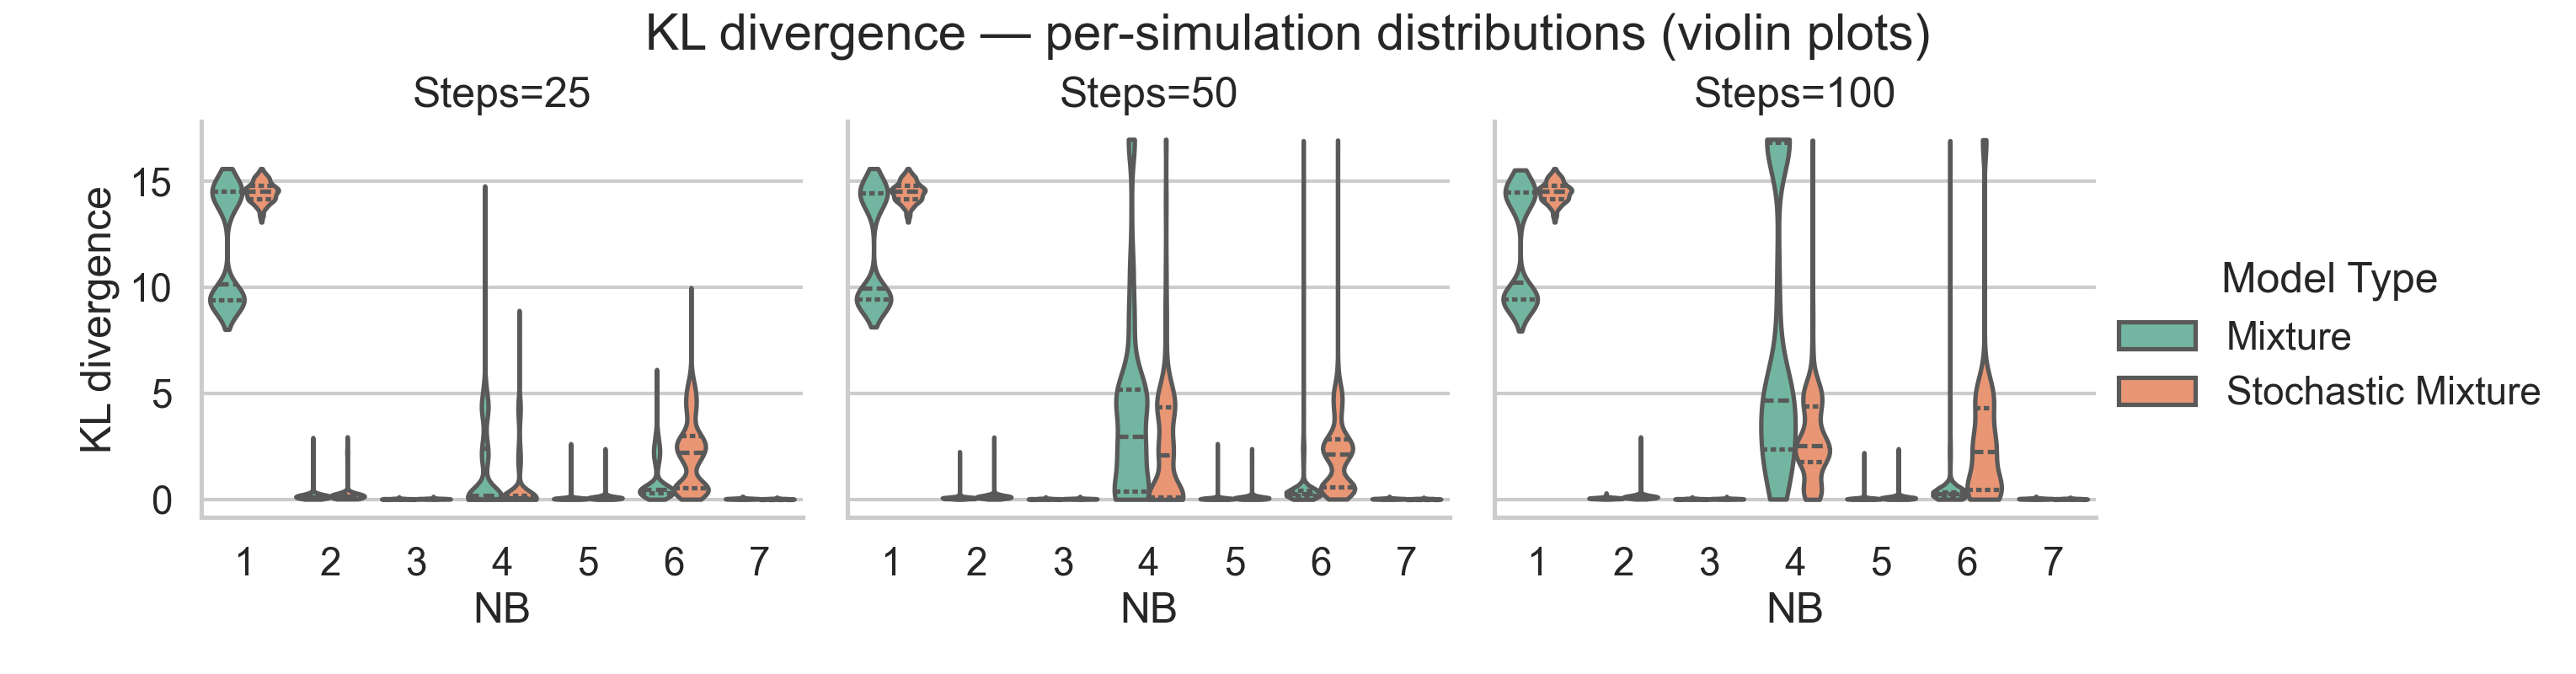
\includegraphics[width=\textwidth]{figs/neighborhood_analysis/nb_sweep_300x100/violin_KL_Divergence.png}
  \caption{Step 3: per-simulation violin plots for KL divergence (lower is better), faceted by step length. Violin width reflects density, and inner quartiles highlight robust central behavior; long upper tails indicate rare but severe failures that become more likely for specific neighborhood sizes and time horizons.}
  \label{fig:impl:step3:violin:kl}
\end{figure}

\begin{figure}[t]
  \centering
  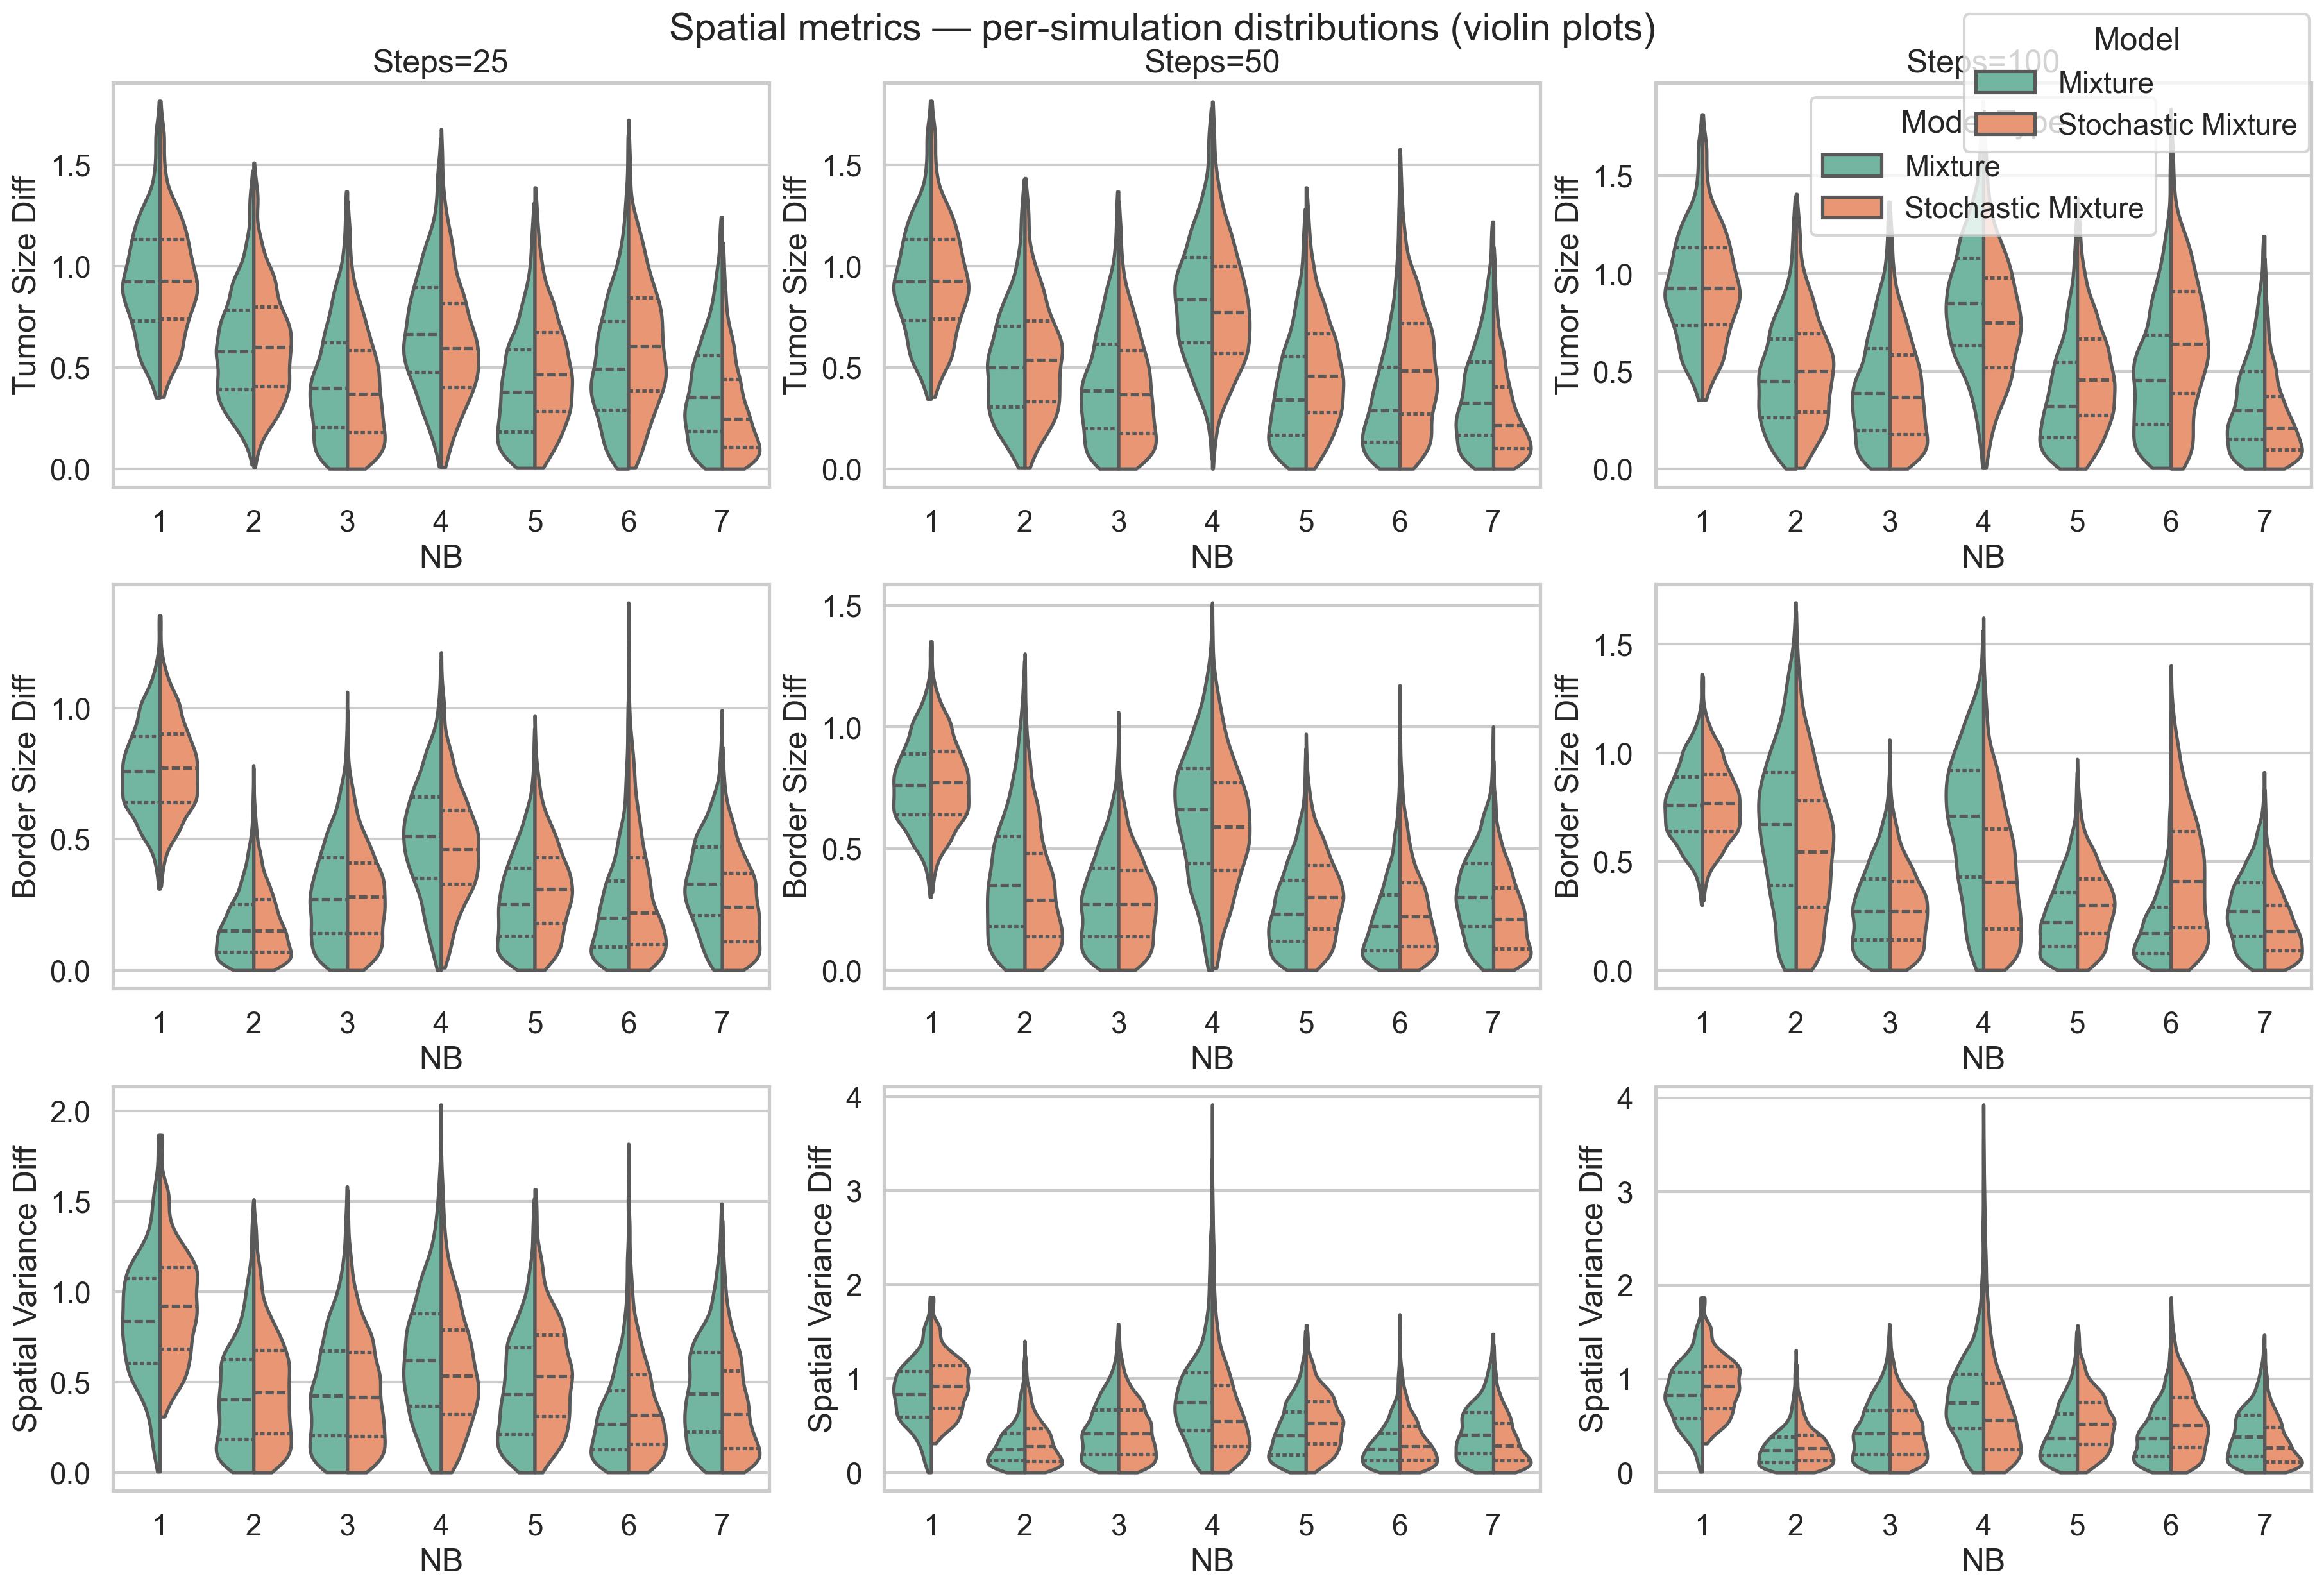
\includegraphics[width=\textwidth]{figs/neighborhood_analysis/nb_sweep_300x100/violin_spatial_metrics.png}
  \caption{Step 3: per-simulation violin plots for spatial metrics (tumor size, border size, spatial variance; lower is better), with one column per step length. This view complements mean trends by explicitly showing variability and tail risk as a function of neighborhood size.}
  \label{fig:impl:step3:violin:spatial}
\end{figure}

%----------------------------------------------------------
\subsubsection{Trend analysis and fold change}
\label{sec:impl:step3:trend}
%----------------------------------------------------------

To summarize how performance changes with neighborhood size in a compact way, we also compute a simple trend analysis over \(NB\).
In particular, we report fold change between a reference neighborhood (here \(NB=3\), used as a normalization point in the sweep) and a larger neighborhood (here \(NB=7\)).
This is useful because in several metrics the main effect is the jump from \(NB=1\) to \(NB\ge2\), while differences among \(NB\ge2\) are smaller and may depend on the metric.

\begin{figure}[t]
  \centering
  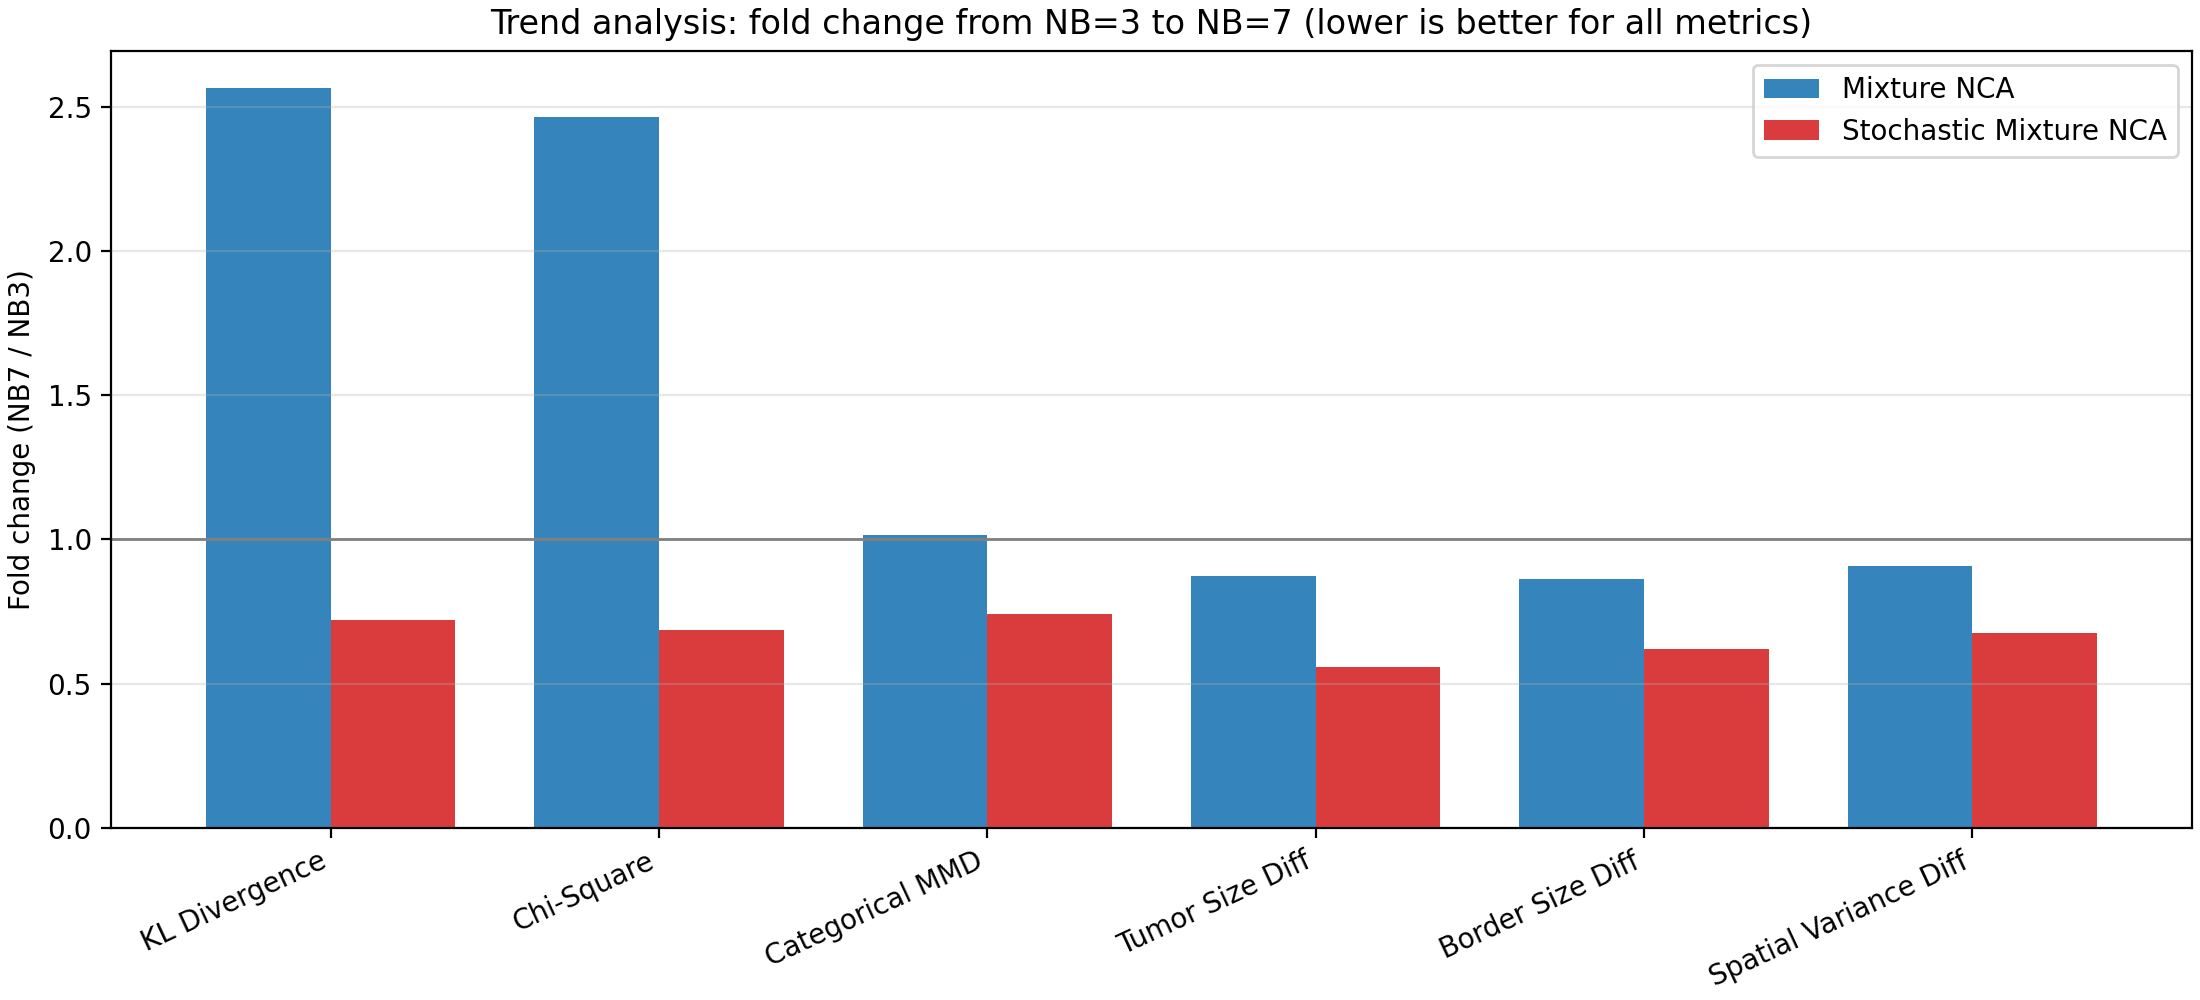
\includegraphics[width=\textwidth]{figs/neighborhood_analysis/nb_sweep_300x100/trend_foldchange_nb7_over_nb3.png}
  \caption{Step 3: trend analysis via fold change from \(NB=3\) to \(NB=7\) (ratio \(\\text{metric}(NB=7)/\\text{metric}(NB=3)\)). Values below 1 indicate improvement when increasing neighborhood size from 3 to 7, while values above 1 indicate degradation.}
  \label{fig:impl:step3:trend:foldchange}
\end{figure}

%----------------------------------------------------------
\subsubsection{Robustness via bad-rate}
\label{sec:impl:step3:badrate}
%----------------------------------------------------------

Mean values alone can hide important instability: per-simulation distributions often show heavy tails where a non-trivial fraction of runs ends in poor outcomes (``failure modes'').
To quantify this, we define a \emph{bad-rate} as follows: for each metric and each (model, step length), we select the neighborhood size with the best median performance, take the 95th percentile of that best distribution as a threshold, and compute for each \(NB\) the probability that a run exceeds this threshold.

\begin{figure}[t]
  \centering
  
\includegraphics[width=\textwidth]{figs/neighborhood_analysis/nb_sweep_300x100/badrate_bars_KL_Divergence.png}
  \caption{Step 3: bad-rate for KL divergence across neighborhood sizes (lower is better). Each bar reports the fraction of per-simulation runs whose KL exceeds the 95th percentile of the best-performing neighborhood for that (model, step length), highlighting robustness differences not visible in means alone.}
  \label{fig:impl:step3:badrate:kl}
\end{figure}

\begin{figure}[t]
  \centering
  
\includegraphics[width=\textwidth]{figs/neighborhood_analysis/nb_sweep_300x100/badrate_bars_Tumor_Size_Diff.png}
  \caption{Step 3: bad-rate for tumor size error (lower is better). Larger neighborhoods generally reduce the probability of severe failures for coarse morphology, especially for the stochastic variant.}
  \label{fig:impl:step3:badrate:tumor}
\end{figure}

\begin{figure}[t]
  \centering
  
\includegraphics[width=\textwidth]{figs/neighborhood_analysis/nb_sweep_300x100/badrate_bars_Border_Size_Diff.png}
  \caption{Step 3: bad-rate for border size error (lower is better). Border-related fidelity exhibits a trade-off: some intermediate neighborhood sizes may show heavier tails, indicating a higher chance of producing unrealistic borders even if the median performance is competitive.}
  \label{fig:impl:step3:badrate:border}
\end{figure}

\begin{figure}[t]
  \centering
  
\includegraphics[width=\textwidth]{figs/neighborhood_analysis/nb_sweep_300x100/badrate_bars_Spatial_Variance_Diff.png}
  \caption{Step 3: bad-rate for spatial variance error (lower is better). Spatial variance is particularly sensitive to step length and neighborhood size, showing that increasing \(NB\) can change both typical behavior and stability of the dynamics.}
  \label{fig:impl:step3:badrate:spvar}
\end{figure}

%----------------------------------------------------------
\subsubsection{Computational complexity and rule specialization}
\label{sec:impl:step3:complexity_rules}
%----------------------------------------------------------

Figure~\ref{fig:impl:step3:complexity} reports the empirical runtime as a function of neighborhood size.
In the explored range \(NB\in[1,7]\), the measured runtime remains approximately flat.
Empirically, Mixture NCA runs at about \(\sim 1.5\) ms/step on average, while the Stochastic Mixture variant is about \(\sim 3.2\) ms/step, with limited variation across neighborhood size.
This suggests that in this implementation range the practical cost is dominated by constants and vectorization effects rather than by the naive theoretical \(O(NB^2)\) scaling.

\begin{figure}[t]
  \centering
  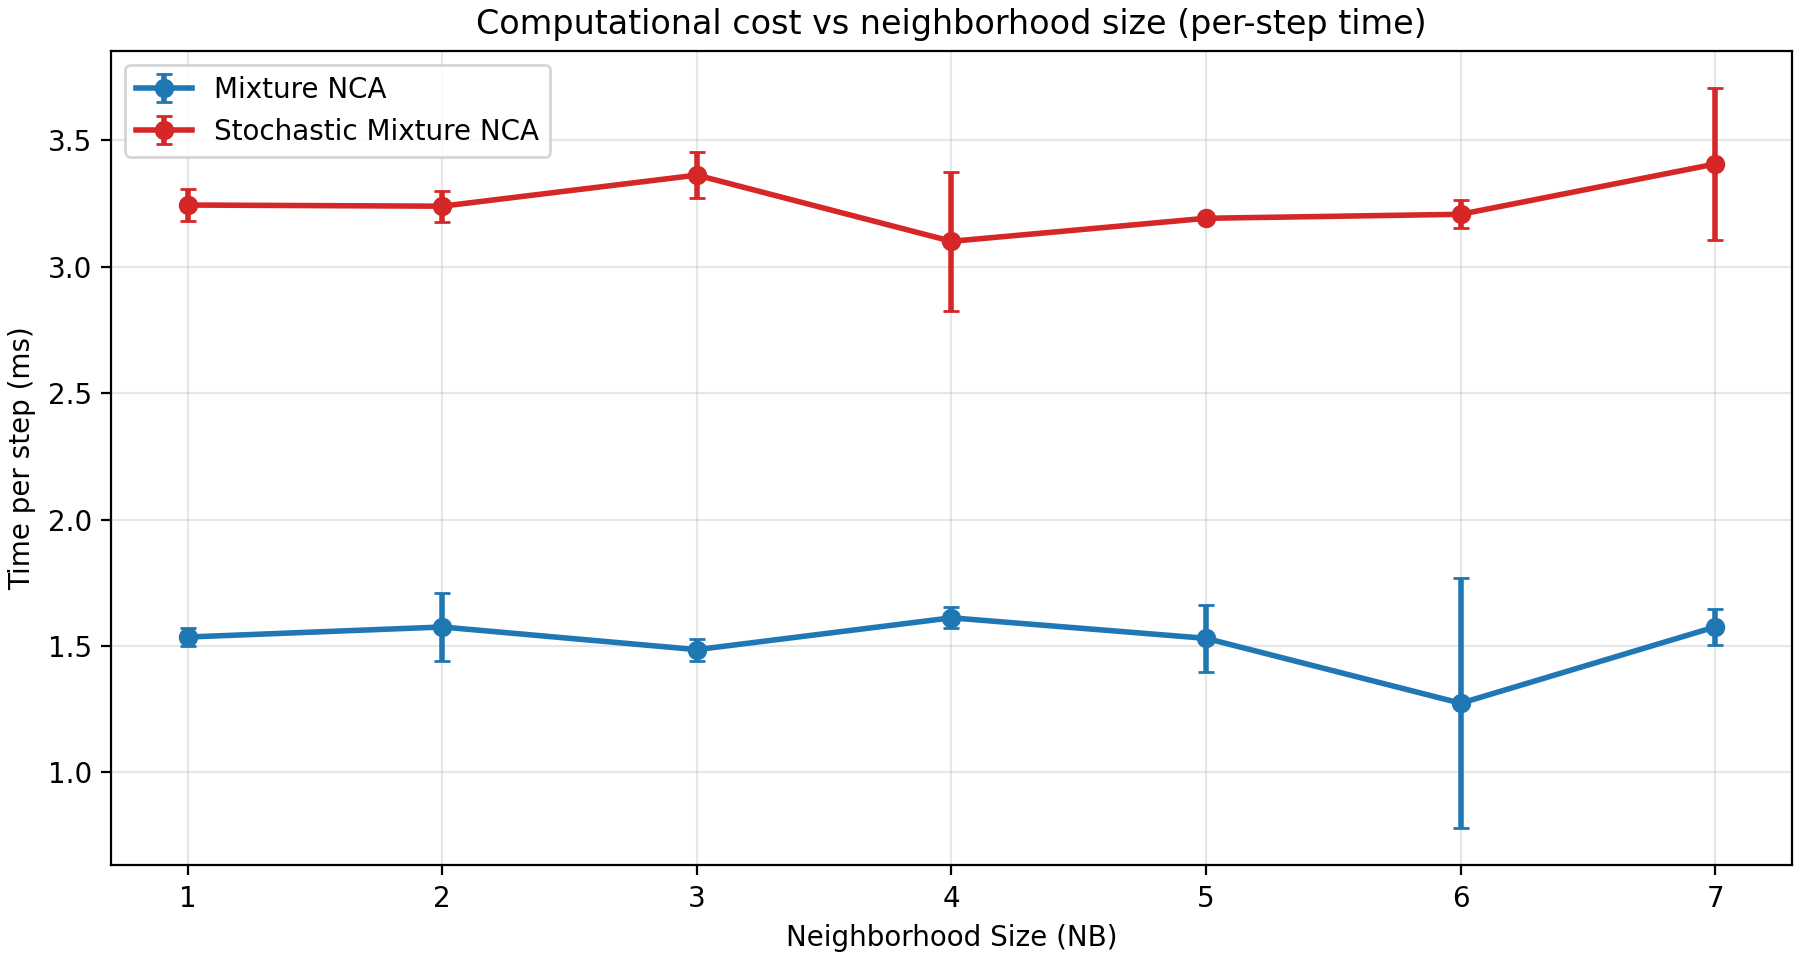
\includegraphics[width=0.85\textwidth]{figs/neighborhood_analysis/nb_sweep_300x100/computational_complexity_time_per_step.png}
  \caption{Step 3: empirical computational cost vs neighborhood size for Mixture and Stochastic Mixture NCA, shown as time per simulation step (ms). Error bars are derived from repeated timing runs.}
  \label{fig:impl:step3:complexity}
\end{figure}

\begin{figure}[t]
  \centering
  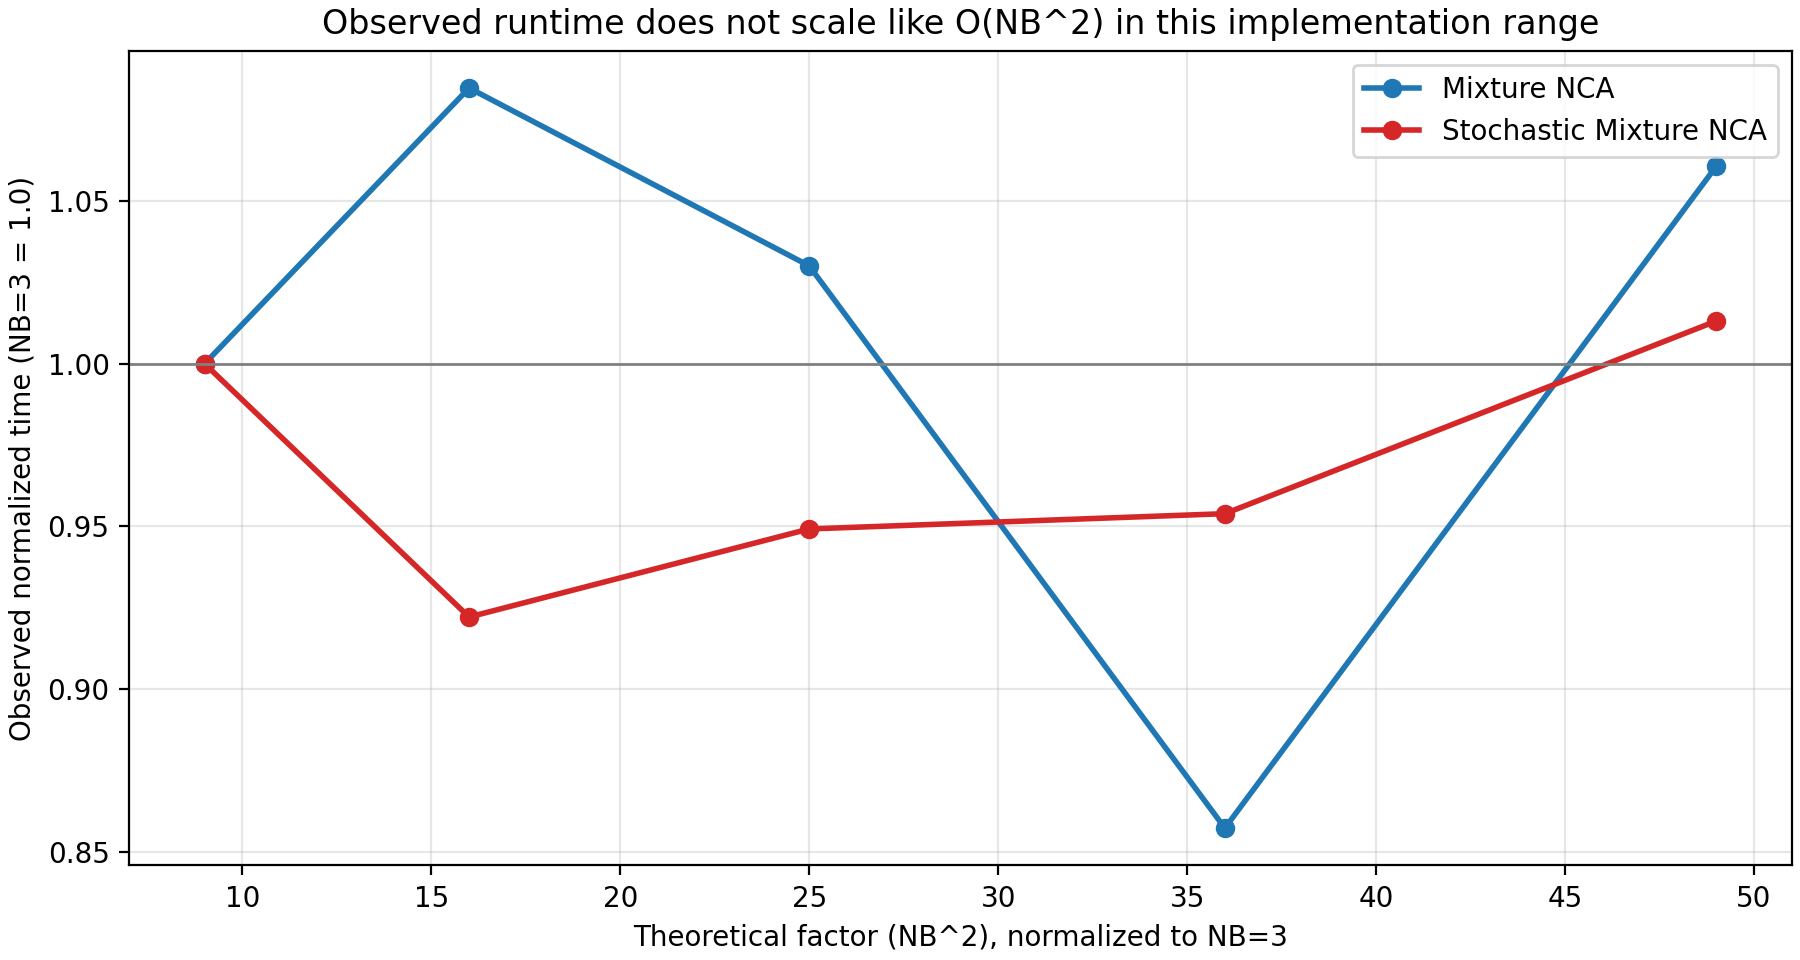
\includegraphics[width=0.85\textwidth]{figs/neighborhood_analysis/nb_sweep_300x100/computational_complexity_normalized_vs_theory.png}
  \caption{Step 3: normalized runtime compared to a theoretical \(NB^2\) scaling. The observed normalized time (relative to \(NB=3\)) stays close to 1.0 and does not increase proportionally to \(NB^2\) in this range.}
  \label{fig:impl:step3:complexity:theory}
\end{figure}

Finally, we analyze how rules are selected over time as a function of neighborhood size, which provides a qualitative explanation for the observed trade-offs and stability differences.
To study how specialization evolves during the dynamics, we measure the entropy of the model's rule-assignment distribution \(p(r \mid x_t)\) at each time step, averaged over space and over sampled simulations.
Low entropy indicates confident (specialized) rule selection, while higher entropy indicates mixed or uncertain rule usage.

\begin{figure}[t]
  \centering
  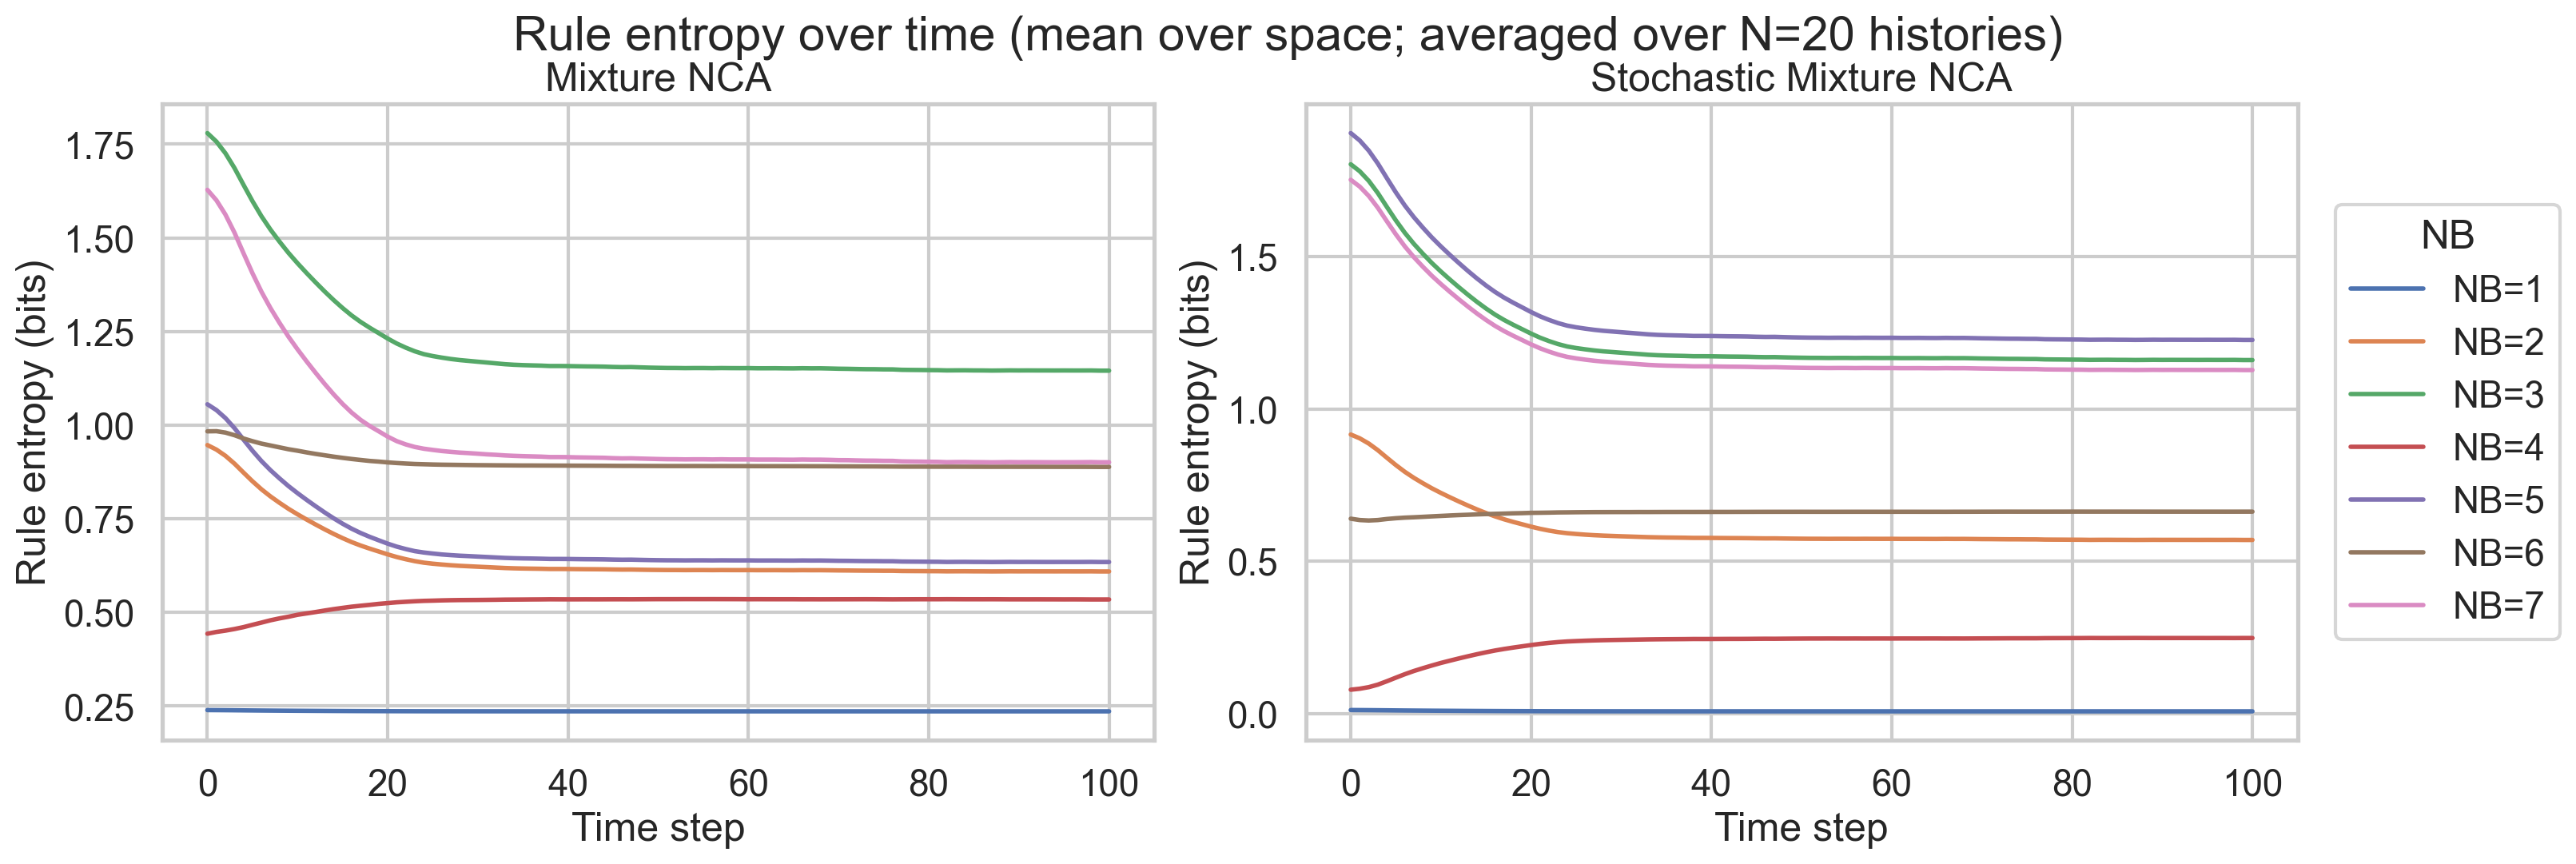
\includegraphics[width=\textwidth]{figs/neighborhood_analysis/nb_sweep_300x100/rule_entropy_over_time.png}
  \caption{Step 3: rule-assignment entropy over time (in bits), averaged over space and across sampled histories (\(N=20\)), for Mixture NCA and Stochastic Mixture NCA on the 300x100 sweep run. Curves correspond to different neighborhood sizes; the temporal profiles highlight how increasing \(NB\) changes the specialization dynamics and can correlate with stability differences.}
  \label{fig:impl:step3:entropy:time}
\end{figure}

\paragraph{Rule specialization summary and interpretation.}
To complement the time-series view, we also summarize rule specialization with three simple indicators:
(i) mean entropy (lower means more confident selection),
(ii) rule diversity (higher means probability mass is spread over more rules),
and (iii) max rule usage (the maximum average probability assigned to a single rule; lower means more balanced usage).
Figure~\ref{fig:impl:step3:rule:summary} reports these indicators and relates them to KL divergence at Step Length \(=100\).

\begin{figure}[t]
  \centering
  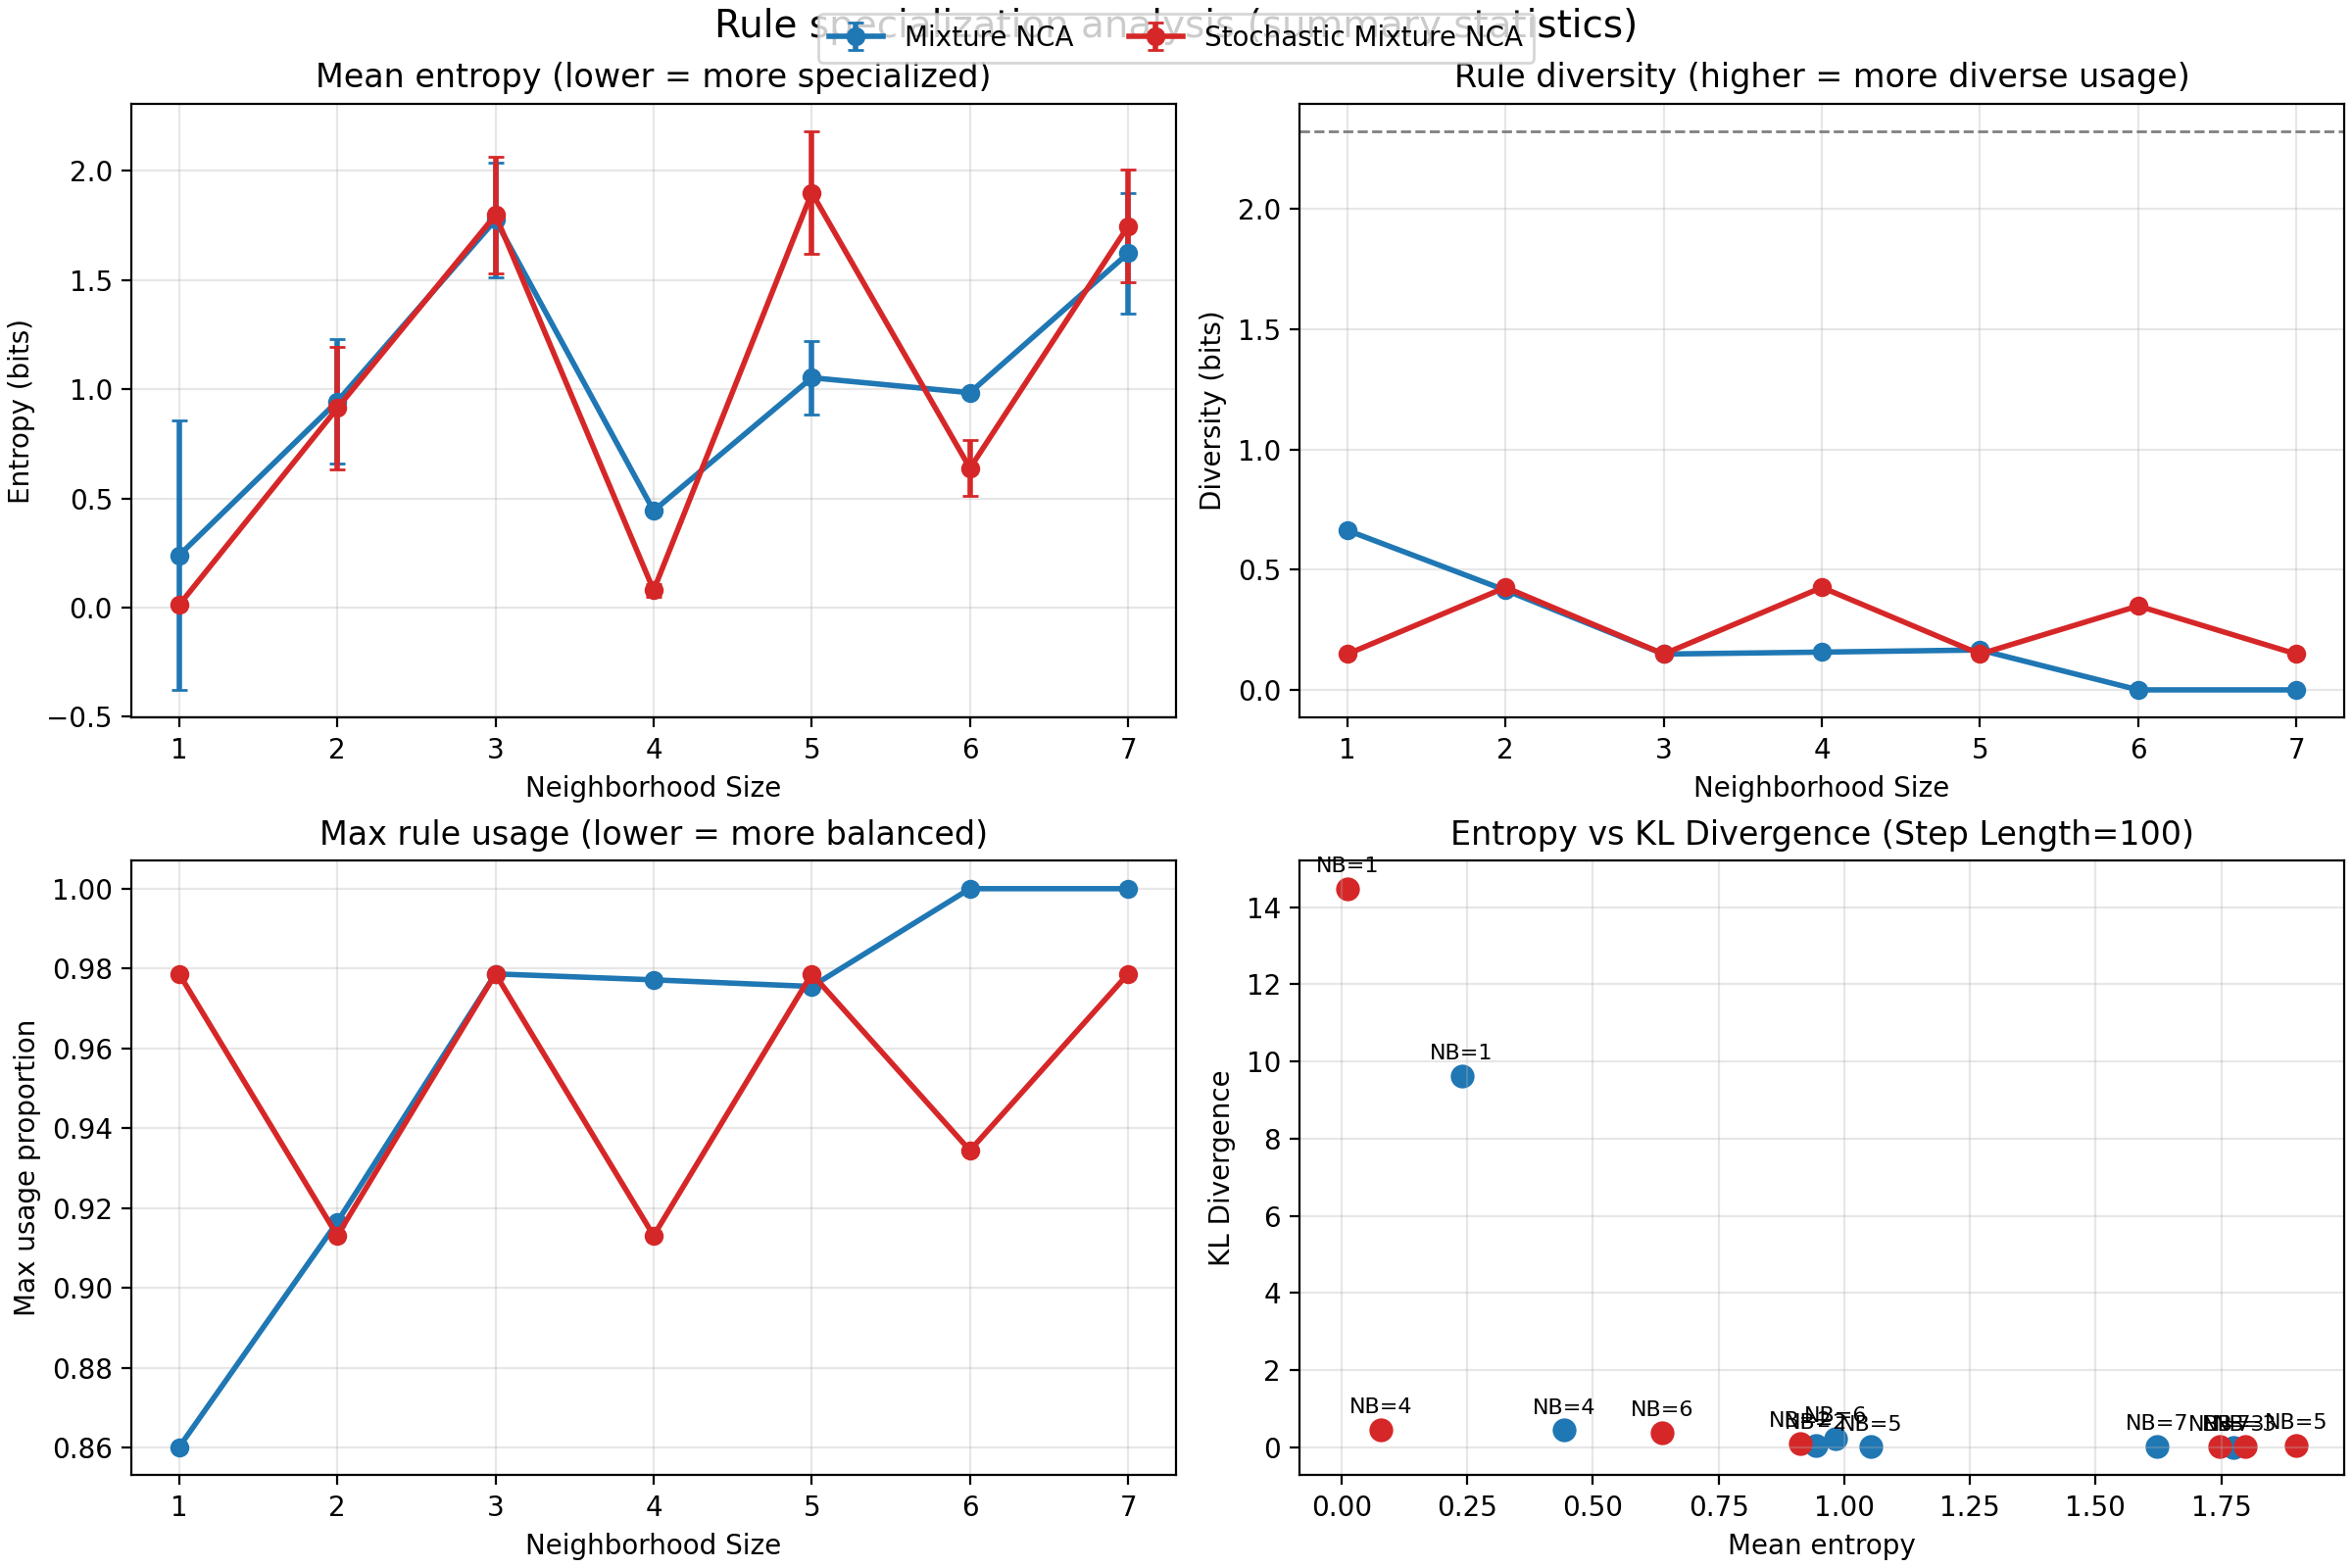
\includegraphics[width=\textwidth]{figs/neighborhood_analysis/nb_sweep_300x100/rule_specialization_summary.png}
  \caption{Step 3: rule specialization summary statistics across neighborhood sizes for Mixture and Stochastic Mixture NCA. The bottom-right panel relates specialization (entropy) to performance (KL divergence) at Step Length \(=100\).}
  \label{fig:impl:step3:rule:summary}
\end{figure}

\paragraph{Rule assignment maps (illustrative examples).}
To make rule selection more intuitive, we visualize the \emph{rule-assignment probability maps} \(p(r \mid x)\) for a single example state.
Each heatmap shows, for each spatial position, how likely the model is to select a given rule.
Figures~\ref{fig:impl:step3:rule:maps:mix} and~\ref{fig:impl:step3:rule:maps:stoch} show examples for selected neighborhood sizes (including small and large \(NB\)).

\begin{figure}[t]
  \centering
  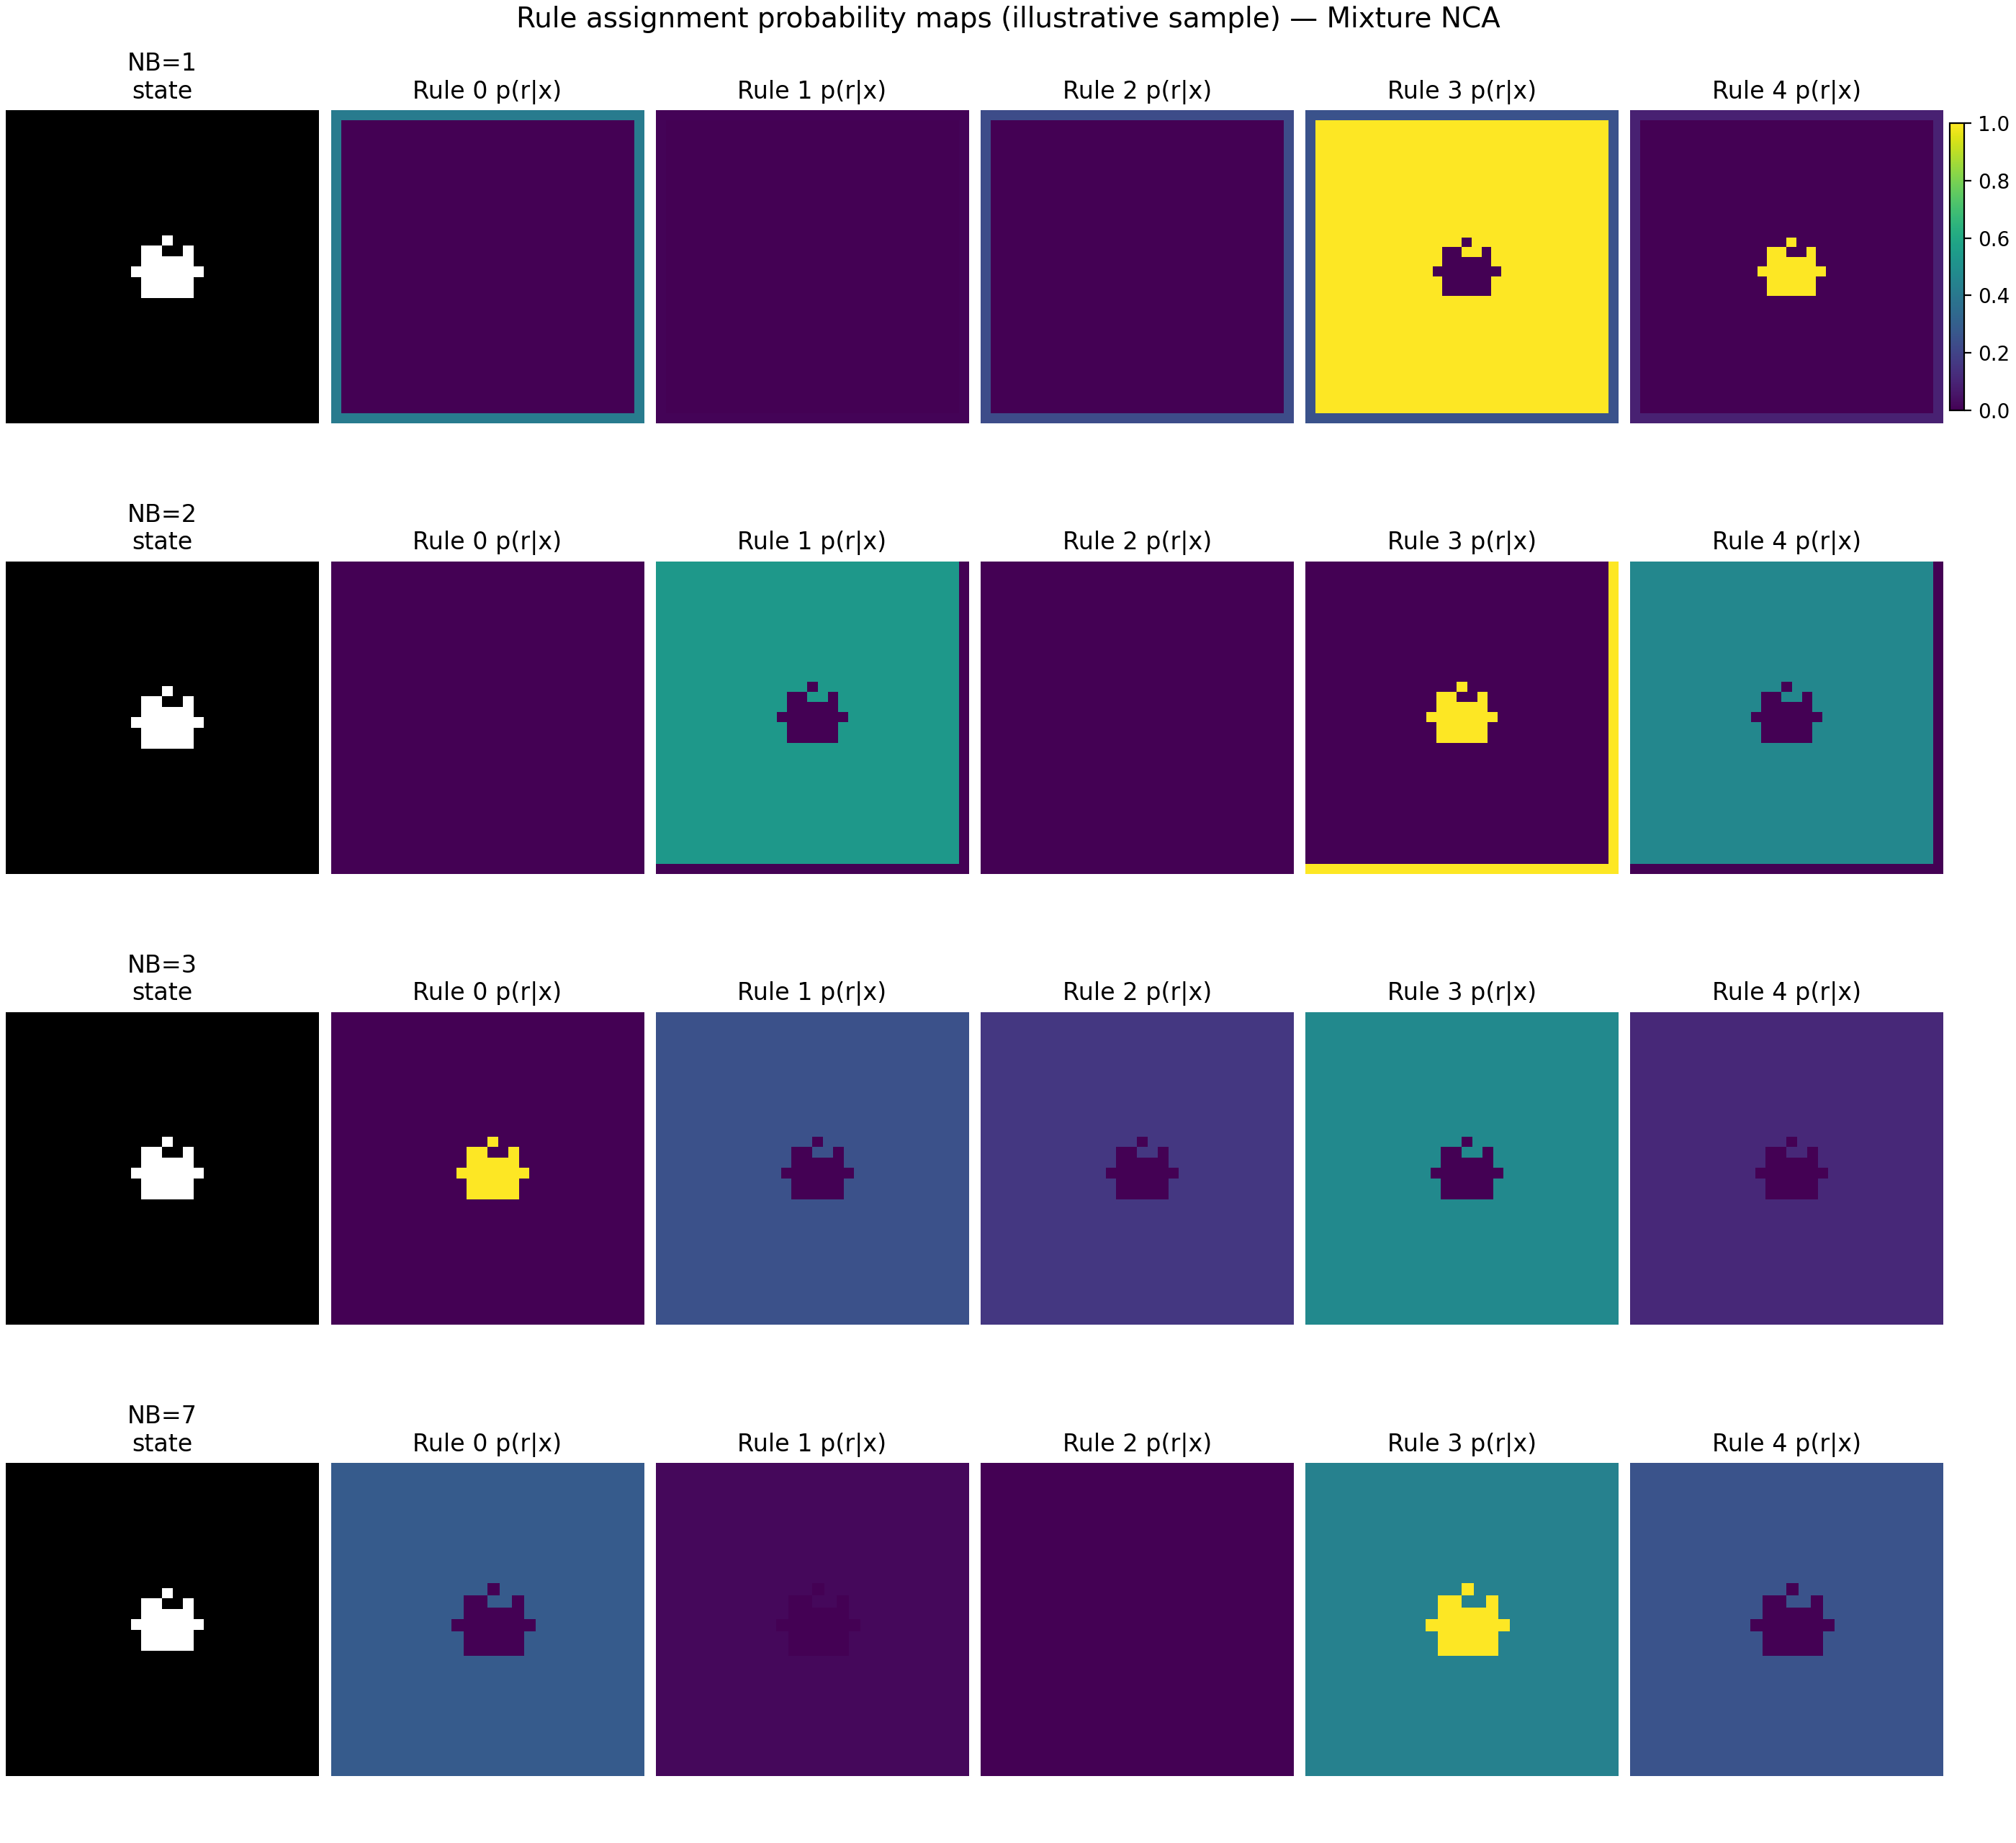
\includegraphics[width=\textwidth]{figs/neighborhood_analysis/nb_sweep_300x100/rule_assignment_maps_mixture.png}
  \caption{Step 3: illustrative rule assignment probability maps for Mixture NCA (one example state). Columns show the input state and the five rule probability maps. Rows correspond to selected neighborhood sizes.}
  \label{fig:impl:step3:rule:maps:mix}
\end{figure}

\begin{figure}[t]
  \centering
  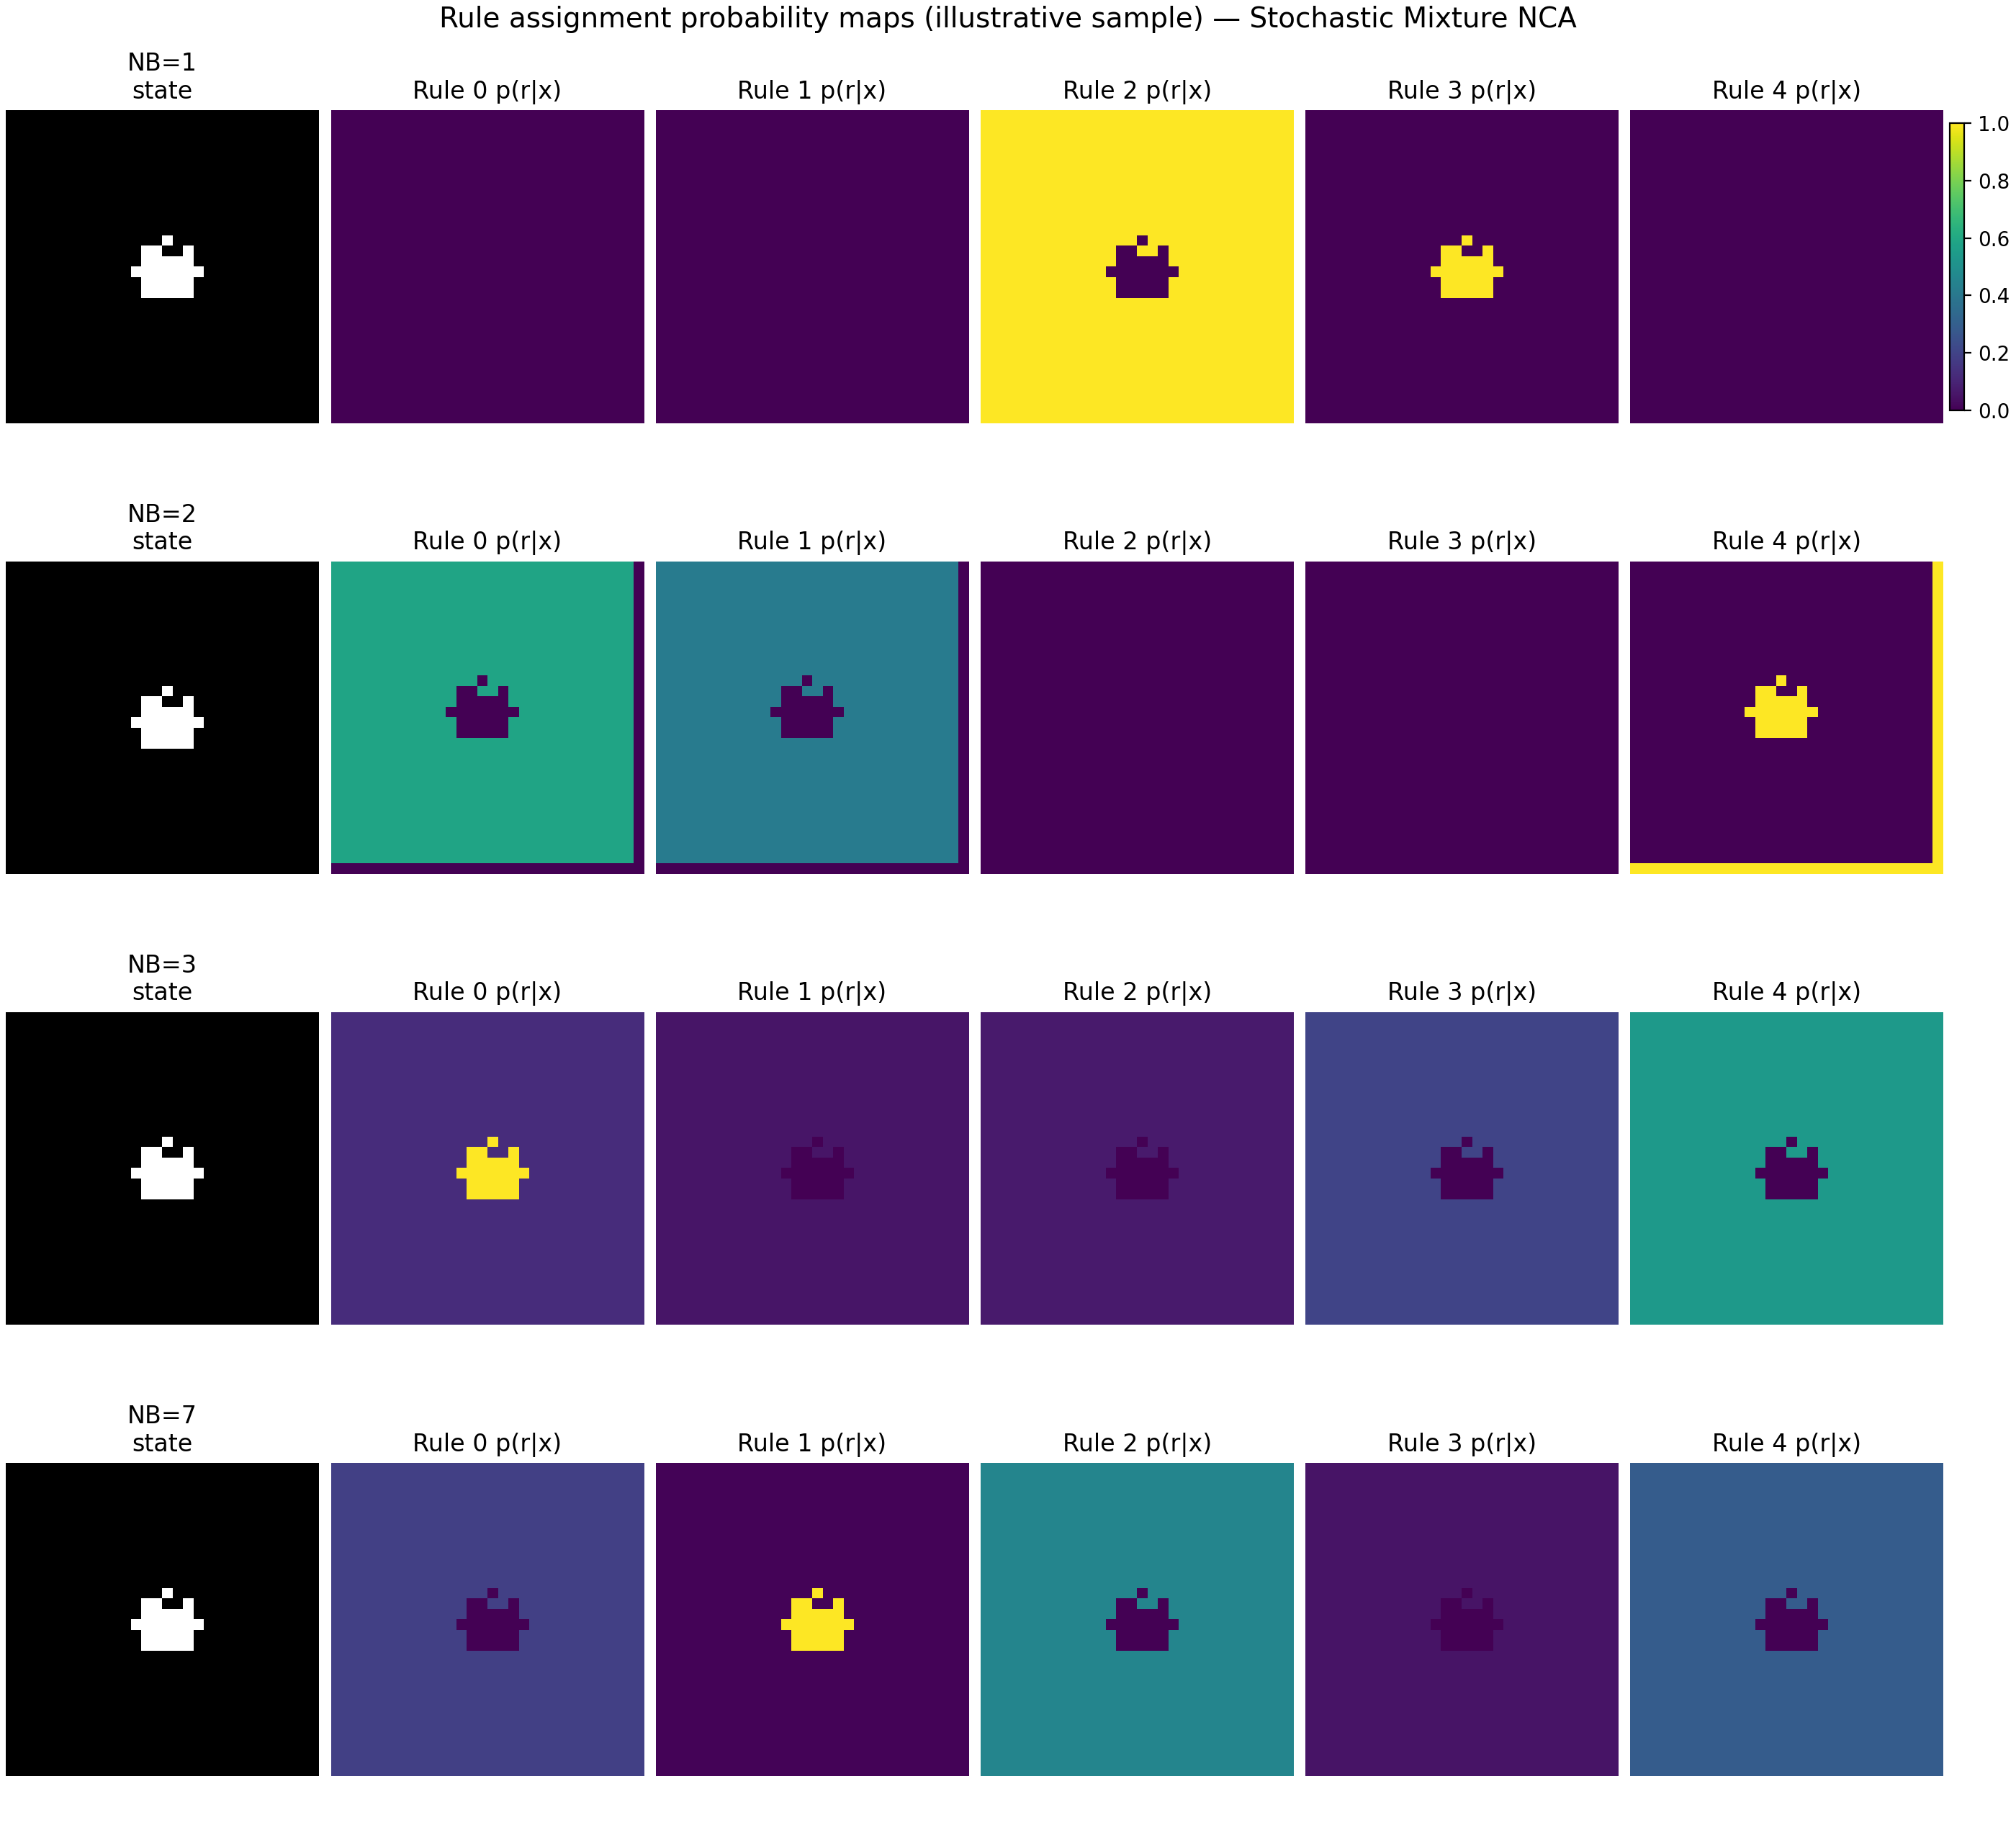
\includegraphics[width=\textwidth]{figs/neighborhood_analysis/nb_sweep_300x100/rule_assignment_maps_stochastic.png}
  \caption{Step 3: illustrative rule assignment probability maps for Stochastic Mixture NCA (one example state). The stochastic variant can exhibit different specialization patterns even when average performance is similar.}
  \label{fig:impl:step3:rule:maps:stoch}
\end{figure}

%----------------------------------------------------------
\subsubsection{Statistical tests (non-parametric)}
\label{sec:impl:step3:stats}
%----------------------------------------------------------

Finally, we add a lightweight statistical check to verify that the observed differences across neighborhood sizes are not explained only by noise.
Because per-simulation metric distributions can be heavy-tailed and not obviously Gaussian, we use non-parametric tests: an overall Kruskal--Wallis test across \(NB\in\{1,\dots,7\}\), followed by post-hoc Mann--Whitney U tests comparing each \(NB\ge2\) against \(NB=1\), with Holm correction within each metric.

% Auto-generated by experiments/generate_step3_stats_table.py
% Statistical tests: Step Length=100, baselines NB=2 and NB=3, Holm correction.
\begin{table}[H]
\centering
\small
\begin{tabulary}{\textwidth}{lLrLL}
\toprule
Model & Metric & Kruskal-Wallis $p$ & Significant vs NB=2 & Significant vs NB=3 \\
\midrule
Mixture~NCA & KL Divergence & $<10^{-4}$ & 3,4,5,6,7 & 4,5,6,7 \\
Mixture~NCA & Chi-Square & $<10^{-4}$ & 3,4,5,6,7 & 4,5,6,7 \\
Mixture~NCA & Categorical MMD & $<10^{-4}$ & 3,4,5,6,7 & 4,5,6 \\
Mixture~NCA & Tumour Size Diff & $<10^{-4}$ & 3,4,5,6,7 & 4,5,6,7 \\
Mixture~NCA & Border Size Diff & $<10^{-4}$ & 3,4,5,6,7 & 4,5,6,7 \\
Mixture~NCA & Spatial Variance Diff & $<10^{-4}$ & 3,4,5,6,7 & 4,5,6,7 \\
Stochastic~Mixture~NCA & KL Divergence & $<10^{-4}$ & 3,4,5,6,7 & 4,5,6,7 \\
Stochastic~Mixture~NCA & Chi-Square & $<10^{-4}$ & 3,4,5,6,7 & 4,5,6,7 \\
Stochastic~Mixture~NCA & Categorical MMD & $<10^{-4}$ & 3,4,5,7 & 4,5,6,7 \\
Stochastic~Mixture~NCA & Tumour Size Diff & $<10^{-4}$ & 3,4,5,7 & 4,5,6,7 \\
Stochastic~Mixture~NCA & Border Size Diff & $<10^{-4}$ & 4,5,6,7 & 4,5,6,7 \\
Stochastic~Mixture~NCA & Spatial Variance Diff & $<10^{-4}$ & 3,4,5,6,7 & 4,5,7 \\
\bottomrule
\end{tabulary}
\caption{Non-parametric statistical tests across neighbourhood sizes for Step Length $=100$. \textbf{Legend:} Model = Mixture NCA or Stochastic Mixture NCA; Metric = one of the six metrics; Kruskal-Wallis $p$ over $NB\in\{1,\dots,7\}$; last two columns = list of $NB$ that differ significantly from baseline $NB=2$ (post-hoc Mann-Whitney U, Holm correction) and from baseline $NB=3$.}
\label{tab:impl:step3:stats}
\end{table}

